%************************************************
\chapter{Background estimation}
\label{ch:BG}
%************************************************

The charge flip background and the fake lepton background are the two dominant backgrounds that their original particles in the final state come from the SM, but not the SUSY signal. Because of the mis-reconstruction, they pass the selections of the SRs. This type of background will be estimated by using the data-driven method.

\section{charge flip background}
\subsection{Sources for charge flip background}
The charge flip background is due to the mis-identification of the sign of the charge of a lepton, after the reconstruction.
The sign of the charge is determined by the direction of the curvature of the track.
There are two main sources for the mis-identification for the direction of the curvature.

The first source is described by the figure \ref{fig:charge_flip_bremsstrahlung}.
It is the case that the lepton interacts with the material of the detector, and a photon is emitted by the process of bremsstrahlung.
The emitted photon further produces a pair of electron and positron, namely the $\gamma$ conversion.
As shown in figure \ref{fig:charge_flip_bremsstrahlung}, if the most of the energy is carried by the positron $e^{+}$ (the purple track), the direction of the curvature of the reconstructed track (the orange track) will be reversed.
Thus, the charge of the lepton is flipped.
Because the amount of this mis-identification depends on the number of hits with the detector, and hence depends on $|\eta|$ of the original track.

\begin{figure}
\centering
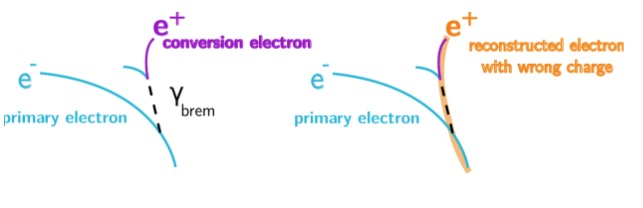
\includegraphics[width=\textwidth]{data/photo/charge_flip/Brem.jpg}
\caption{This shows how the track of the electron is incorrectly reconstructed (the orange track), due to the process of bremsstrahlung and $\gamma$ conversion.}
\label{fig:charge_flip_bremsstrahlung}
\end{figure}

The second source is described by the figure \ref{fig:charge_flip_high_pt}.
When the $p_T$ of the lepton is very high, the track of the lepton will be almost a straight line.
The curvature of the track will be close to zero, and the sign of the curvature will be difficult to distinguish.
As a result, the sign of the charge of the lepton will be incorrectly assigned.
The chance to have this problem obviously depends on $p_T$ of the lepton.

\begin{figure}
\centering
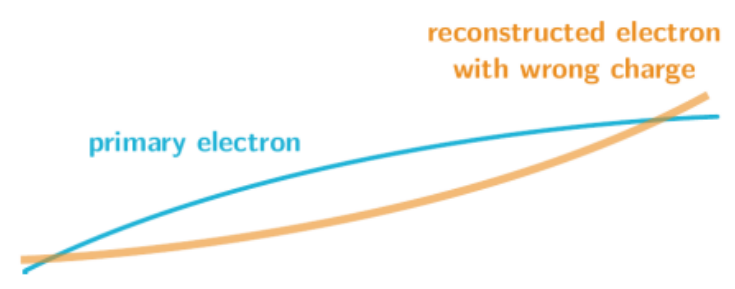
\includegraphics[width=\textwidth]{data/photo/charge_flip/WrongTrack.png}
\caption{This shows how the track of the electron is incorrectly reconstructed (the orange track), due to very high $p_T$ of the electron.}
\label{fig:charge_flip_high_pt}
\end{figure}

Compared to an electron, the charge of a reconstructed muon will be less often to be mis-identified.
The first reason is that a muon is heavier than an electron.
This will reduce the chance of the process of bremsstrahlung.
The second reason is that muons can reach to the muon spectrometer, which is the outer part of the detector, while most electrons cannot.
This means that the length of the track of a muon, which can be detected by the tracker, is longer than that of an electron.
Hence, the reconstructed curvature of the track for muons can be more accurate, and it reduces the chance of the mis-identification due to the high $p_T$.
Becasue most of the charge flip background comes from electrons, we only estimate the charge flip background for electrons.

\subsection{Likelihood method}
\label{sec:likelihood_method}
The probability that the charge of an electron is mis-identified is denoted by the charge-flip rate $\epsilon_i$, where the index i represents the dependency on the $p_T$ and $\eta$ of the electron.
The value of index i is found by splitting the variables $p_T$ and $|\eta|$ into different 2-dimensional bins, and the binning for the $p_T$ and $|\eta|$ is described by the table \ref{table:binning}. The index i of $\epsilon_i$ is defined by the index of the bin.

\begin{table}[htbp]
\centering
\begin{tabular}{|c|c|}
\hline
Variable & Boundary of the bins \\
\hline
$p_T$ (GeV) &  25, 60, 90, 130, 150, 1000 \\
\hline
$|\eta|$ & 0, 0.50, 1.00, 1.37, 1.52, 1.80, 2.00, 2.47 \\
\hline
\end{tabular}
\caption{Binning in $p_T$ and $|\eta|$ for the charge-flip rate $\epsilon_i$.}
\label{table:binning}
\end{table}

Suppose that, before the reconstruction, there are $m^{ij}_{OS}$ opposite-sign events with the leading lepton in bin $i$ and the subleading lepton in bin $j$, and similarly there are $m^{ij}_{SS}$ same-sign events.
After the reconstruction, due to the charge flip, there are $M^{ij}_{OS}$ opposite-sign events and $M^{ij}_{SS}$ same-sign events.
The number of events after the reconstruction is given by
\begin{equation}
M^{ij}_{OS} = (1-\epsilon_i) (1-\epsilon_j) m^{ij}_{OS} + \epsilon_i (1-\epsilon_j) m^{ij}_{SS} + (1-\epsilon_i) \epsilon_j m^{ij}_{SS} + \epsilon_i \epsilon_j m^{ij}_{OS}
\end{equation}
\begin{equation}
M^{ij}_{SS} = (1-\epsilon_i) (1-\epsilon_j) m^{ij}_{SS} + \epsilon_i (1-\epsilon_j) m^{ij}_{OS} + (1-\epsilon_i) \epsilon_j m^{ij}_{OS} + \epsilon_i \epsilon_j m^{ij}_{SS}
\label{equ:MSS}
\end{equation}
From equation \ref{equ:MSS}, the number of reconstructed same-sign events due to the real opposite-sign events, i.e. the charge flip BG , denoted by $N^{ij}_{SS}$, is
\begin{equation}
N^{ij}_{SS} = \epsilon_i (1-\epsilon_j) m^{ij}_{OS} + (1-\epsilon_i) \epsilon_j m^{ij}_{OS}
\label{equ:NSS}
\end{equation}
In the SRs, $m^{ij}_{OS}$ is the number of OS events before the reconstruction, but finally pass all selections in SRs.
$M^{ij}_{OS}$ is the total number of events that pass all selections in SRs, but replace SS requirement by OS.
Because $m^{ij}_{OS}$ is much larger than $m^{ij}_{SS}$ and the measured charge-flip rate $\epsilon_i$ is about $10^{-3}$, $m^{ij}_{OS}$ can be estimated by
\begin{align}
M^{ij}_{OS} &\approx (1-\epsilon_i) (1-\epsilon_j) m^{ij}_{OS} \\
m^{ij}_{OS} &\approx \frac{ M^{ij}_{OS} }{ (1-\epsilon_i) (1-\epsilon_j) }
\label{equ:mapp1} \\
m^{ij}_{OS} &\approx M^{ij}_{OS} \\
m^{ij}_{OS} &\approx M^{ij}_{OS} + M^{ij}_{SS}
\label{equ:mapp2}
\end{align}
By substituting equation \ref{equ:mapp2} into \ref{equ:NSS}, the charge flip BG can be estimated by $M^{ij}_{OS}$, $M^{ij}_{SS}$ and the charge-flip rate $\epsilon_i$,
\begin{align}
N^{ij}_{SS} &= \epsilon_i (1-\epsilon_j) m^{ij}_{OS} + (1-\epsilon_i) \epsilon_j m^{ij}_{OS} \\
&= [ \epsilon_i (1-\epsilon_j) + (1-\epsilon_i) \epsilon_j ] m^{ij}_{OS} \label{equ:NSS3}\\
&\approx p_{ij} (M^{ij}_{OS} + M^{ij}_{SS}) \\
&=p_{ij} N^{ij}
\label{equ:NSS2}
\end{align}
where $p_{ij}$ and $N^{ij}$ are
\begin{align}
\begin{split}
p_{ij} &= \epsilon_i (1-\epsilon_j) + (1-\epsilon_i) \epsilon_j \\
N^{ij} &= M^{ij}_{OS} + M^{ij}_{SS}
\end{split}
\end{align}
The probability density function of $N^{ij}_{SS}$, with the given values of $N^{ij}$ and $\epsilon_i$, can be described by the Poisson distribution with the mean value $\lambda = p_{ij} N^{ij}$.
\begin{align}
P(N^{ij}_{SS}|N^{ij},\epsilon_i,\epsilon_j) &= \frac{ \lambda^{N^{ij}_{SS}} e^{-\lambda} }{N^{ij}_{SS}!} \\
 &= \frac{ (p_{ij} N^{ij})^{N^{ij}_{SS}} e^{- p_{ij} N^{ij}} }{N^{ij}_{SS}!}
\label{equ:poisson}
\end{align}

In order to estimate the charge flip BG, we need to measure the charge-flip rate $\epsilon_i$.
The charge-flip rate is measured as a function of $p_T$ and $|\eta|$ by using a likelihood method, based on the 2015 and 2016 data.
A control region is used to select $Z \rightarrow ee$ processes.
Inside the control region, exactly 2 signal electrons are required.
Also, a Z mass window of 80 GeV $<m_{ll}<$100 GeV is used.
In this control region, the total number of events $N^{ij}$ and the SS events $N^{ij}_{SS}$ in each bin can be measured.
By using the equation \ref{equ:poisson}, the charge-flip rate $\epsilon_i$ can be measured by using the following likelihood method.

The likelihood function $L$ is defined by
\begin{align}
L(\epsilon_i,\epsilon_j|N^{ij},N^{ij}_{SS}) &= \prod_{ij} P(N^{ij}_{SS}|N^{ij},\epsilon_i,\epsilon_j) \\
&= \prod_{ij} \frac{ (p_{ij} N^{ij})^{N^{ij}_{SS}} e^{- p_{ij} N^{ij}} }{N^{ij}_{SS}!} \\
\end{align}
Given the measured values of $N^{ij}$ and $N^{ij}_{SS}$ in each bin, by maximizing the likelihood function over all possible values of $\epsilon_i$, the value of $\epsilon_i$ can be estimated.
By taking the nagative logarithm, it is equivalent to minimize $- \ln L$.
\begin{align}
- \ln L
&= - \ln \prod_{ij} \frac{ (p_{ij} N^{ij})^{N^{ij}_{SS}} e^{- p_{ij} N^{ij}} }{N^{ij}_{SS}!} \\
&= - \sum_{ij} \ln \frac{ (p_{ij} N^{ij})^{N^{ij}_{SS}} e^{- p_{ij} N^{ij}} }{N^{ij}_{SS}!} \\
&= - \sum_{ij} \Big[ N^{ij}_{SS} \ln (p_{ij} N^{ij}) - p_{ij} N^{ij} - \ln( N^{ij}_{SS}!) \Big] \\
&= - \sum_{ij} \Big[ N^{ij}_{SS} \ln (p_{ij} N^{ij}) - p_{ij} N^{ij} \Big] + \text{constant} \\
&= - \sum_{ij} \Big[ N^{ij}_{SS} \ln (N^{ij}[\epsilon_i (1-\epsilon_j) + (1-\epsilon_i) \epsilon_j]) - N^{ij}[\epsilon_i (1-\epsilon_j) + (1-\epsilon_i) \epsilon_j] \Big] + \text{constant}
\end{align}

\subsection{Background substraction}
\label{sec:Background_substraction}
By minimizing $- \ln L$ described in the previous section, the value of the charge-flip rate $\epsilon_i$ can be measured by using the data in the control region.
In order to have better input values of $N^{ij}$ and $N^{ij}_{SS}$, the number of events should mainly come from $Z \rightarrow ee$ processes, and other processes should be substracted.
The number of events from other processes can be estimated by the sideband region: 60 GeV $<m_{ll}<$ 80 GeV and 100 GeV $<m_{ll}<$ 120 GeV.
The corrected values of $N^{ij}$ and $N^{ij}_{SS}$ are given by
\begin{align}
N_{80,100;\text{corrected}} = N_{80,100} - 20 \Big( \frac{N_{60,80} + N_{80,100}}{20 + 20} \Big)
\end{align}
In the sideband substraction, the number of events in the sideband region should be normalized to the width of the central region.
In general, given the number of events in the central region $N_{\text{central}}$, the left sideband region $N_{\text{left}}$ and the right sideband region $N_{\text{right}}$, and their corresponding width $w_{\text{central}}$, $w_{\text{left}}$ and $w_{\text{right}}$, the corrected values $N_{\text{central,corrected}}$ are given by
\begin{align}
N_{\text{central,corrected}} = N_{\text{central}} - w_{\text{central}} \Big( \frac{N_{\text{left}} + N_{\text{right}}}{w_{\text{left}} + w_{\text{right}}} \Big)
\end{align}

\subsection{Results without systematic uncertainty}
\label{sec:results_stat}
Figure \ref{fig:charge_flip_data_stat} shows the measured values of the charge-flip rate $\epsilon_i$ by using the data.
The errors only include the uncertainties in the likelihood method due to the statistics, denoted by $\epsilon_{\text{lik,data}}$.

\begin{figure}
\centering
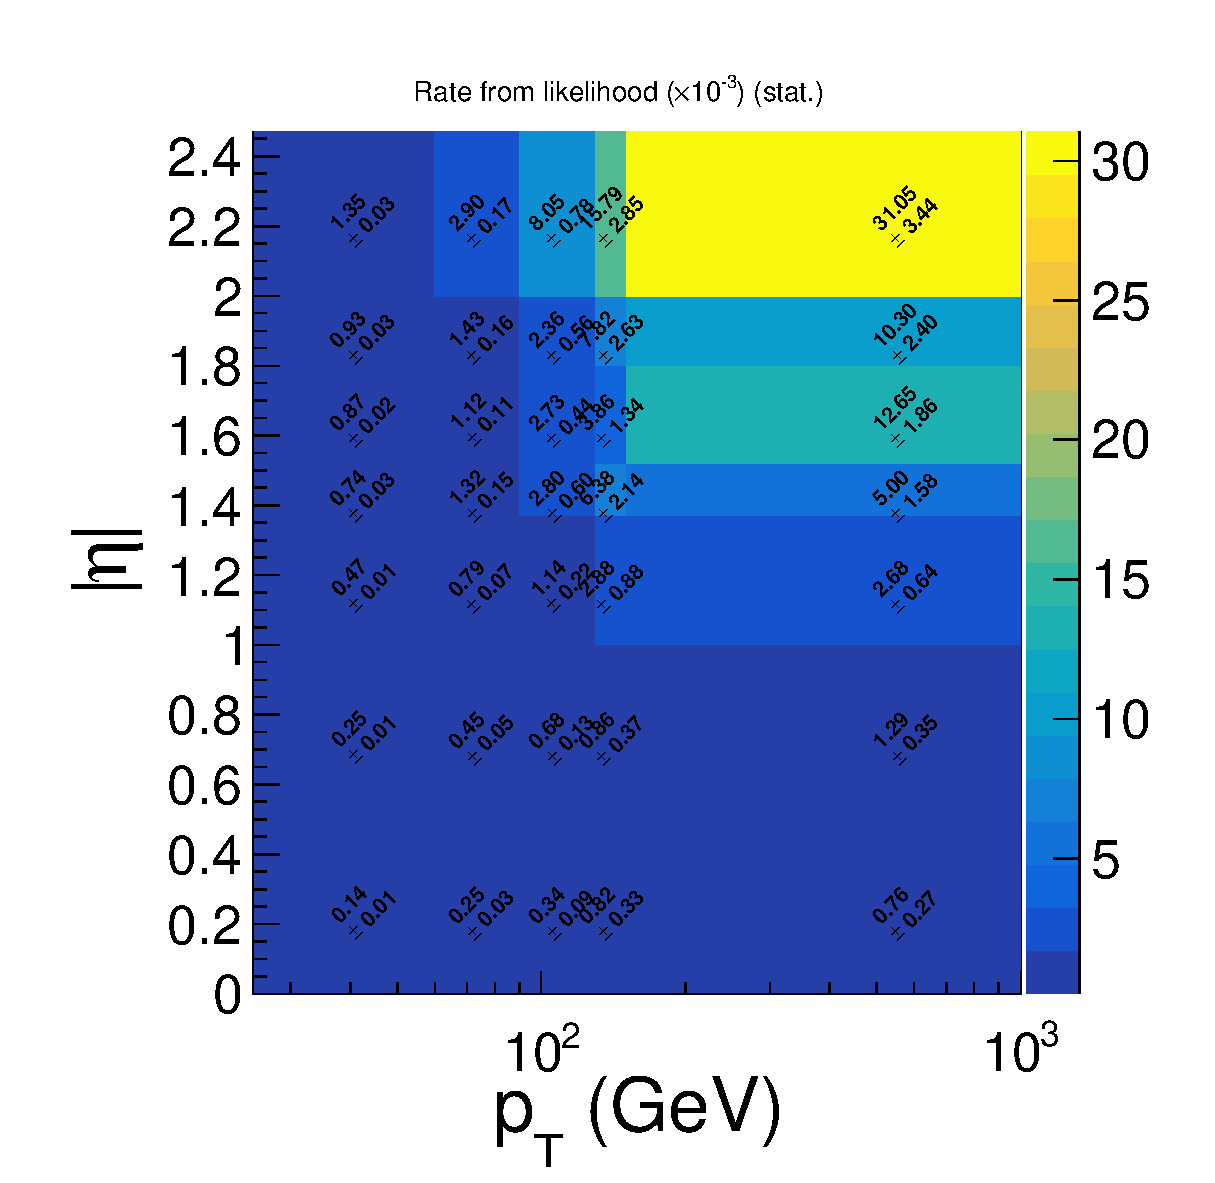
\includegraphics[width=\textwidth]{data/plot/charge_flip/FitPlots/data_cf_rate_stat.eps}
\caption{The measured values of the charge-flip rate $\epsilon_i$ in data. Only uncertainties due to the likelihood method are included.}
\label{fig:charge_flip_data_stat}
\end{figure}

\subsection{Systematic uncertainties due to background substraction}
\label{sec:sys_background_substraction}
The systematic uncertainties due to background substraction is estimated by the variations of different central widths and sideband widths.
The following are the nominal central region and sideband rigion, and their 4 variations. \\
The nominal background substraction:
\begin{itemize}
\item Central region: 80 - 100 GeV; Sideband width: 20 GeV
\end{itemize}
The 4 variations for background substraction:
\begin{itemize}
\item Central region: 80 - 100 GeV; Sideband width: 15 GeV
\item Central region: 80 - 100 GeV; Sideband width: 25 GeV
\item Central region: 75 - 105 GeV; Sideband width: 20 GeV
\item Central region: 80 - 100 GeV; no background subtraction
\end{itemize}

For each bin, the largest deviation from the nominal among these variations is the systematic uncertainty due to background substraction.
\begin{equation}
\sigma_{\text{bgk}} = \max \{| \sigma_{\text{nominal}} - \sigma_{\text{variation}} |\}
\end{equation}

Figure \ref{fig:charge_flip_sys_background_substraction} shows the variations of the resulting charge flip rate, due to these 4 variations.
\begin{figure}
\centering
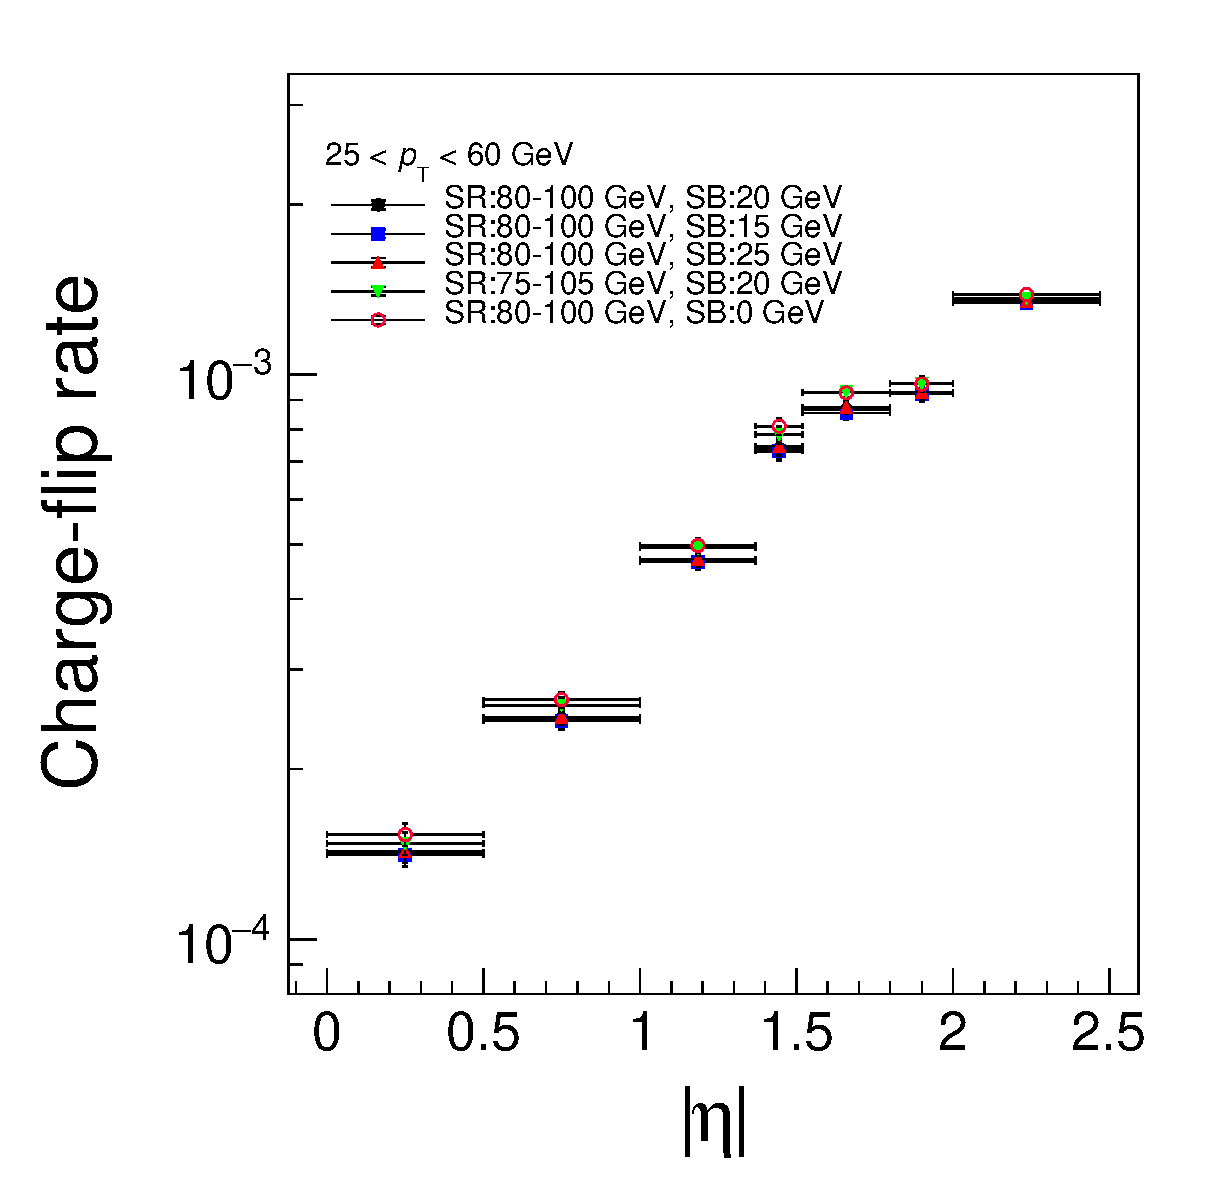
\includegraphics[width=0.3\textwidth]{data/plot/charge_flip/FitPlots/data_cf_comparison_0.eps}
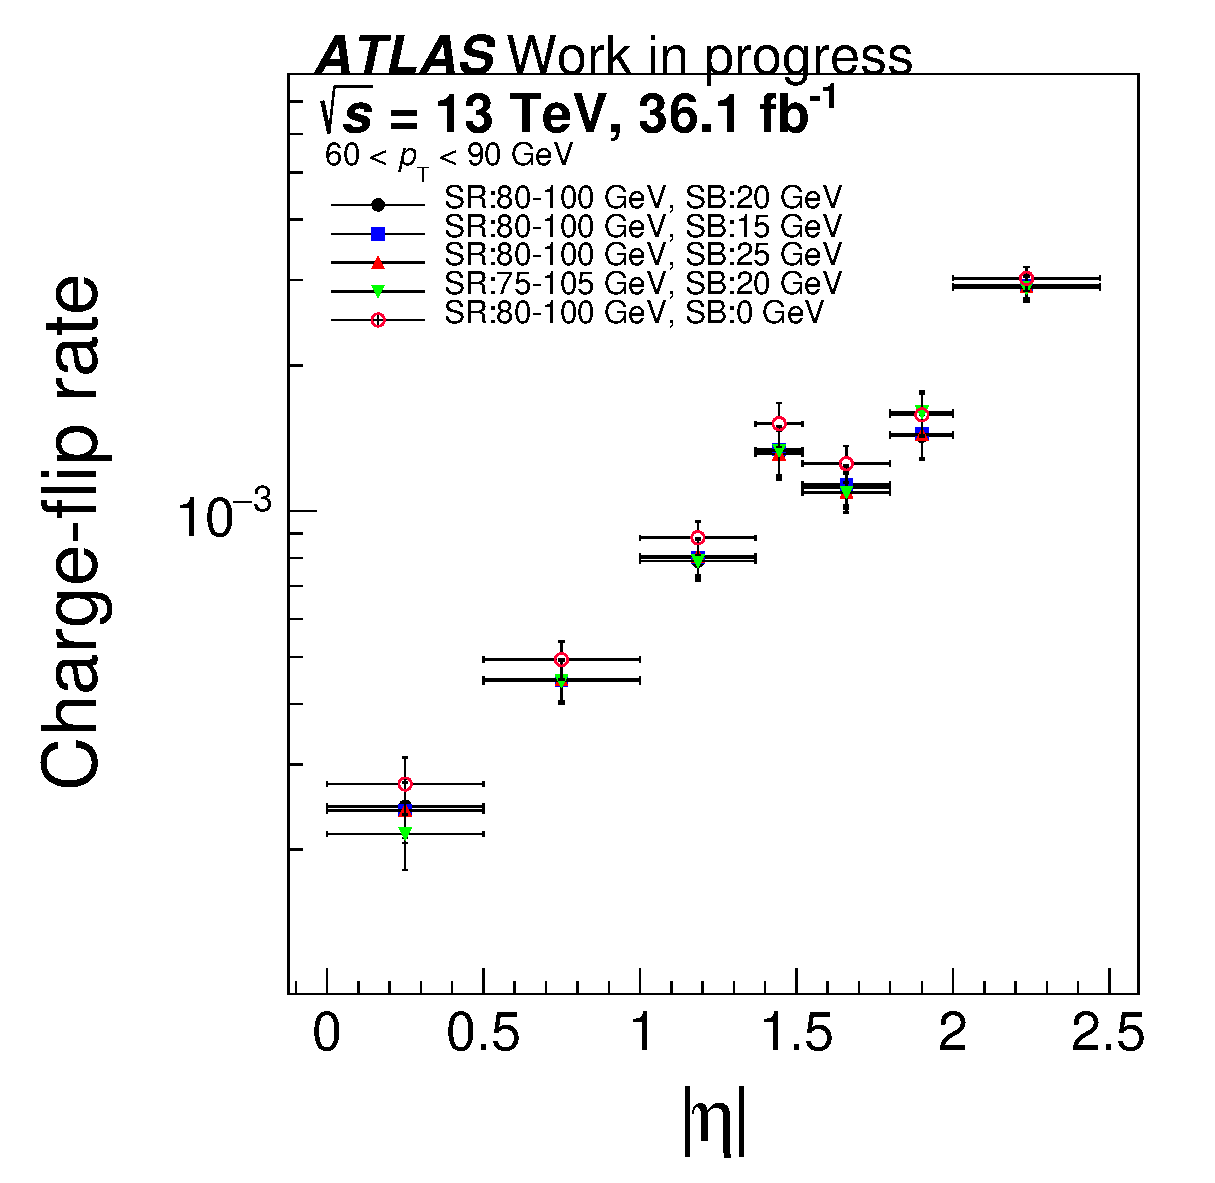
\includegraphics[width=0.3\textwidth]{data/plot/charge_flip/FitPlots/data_cf_comparison_1.eps}
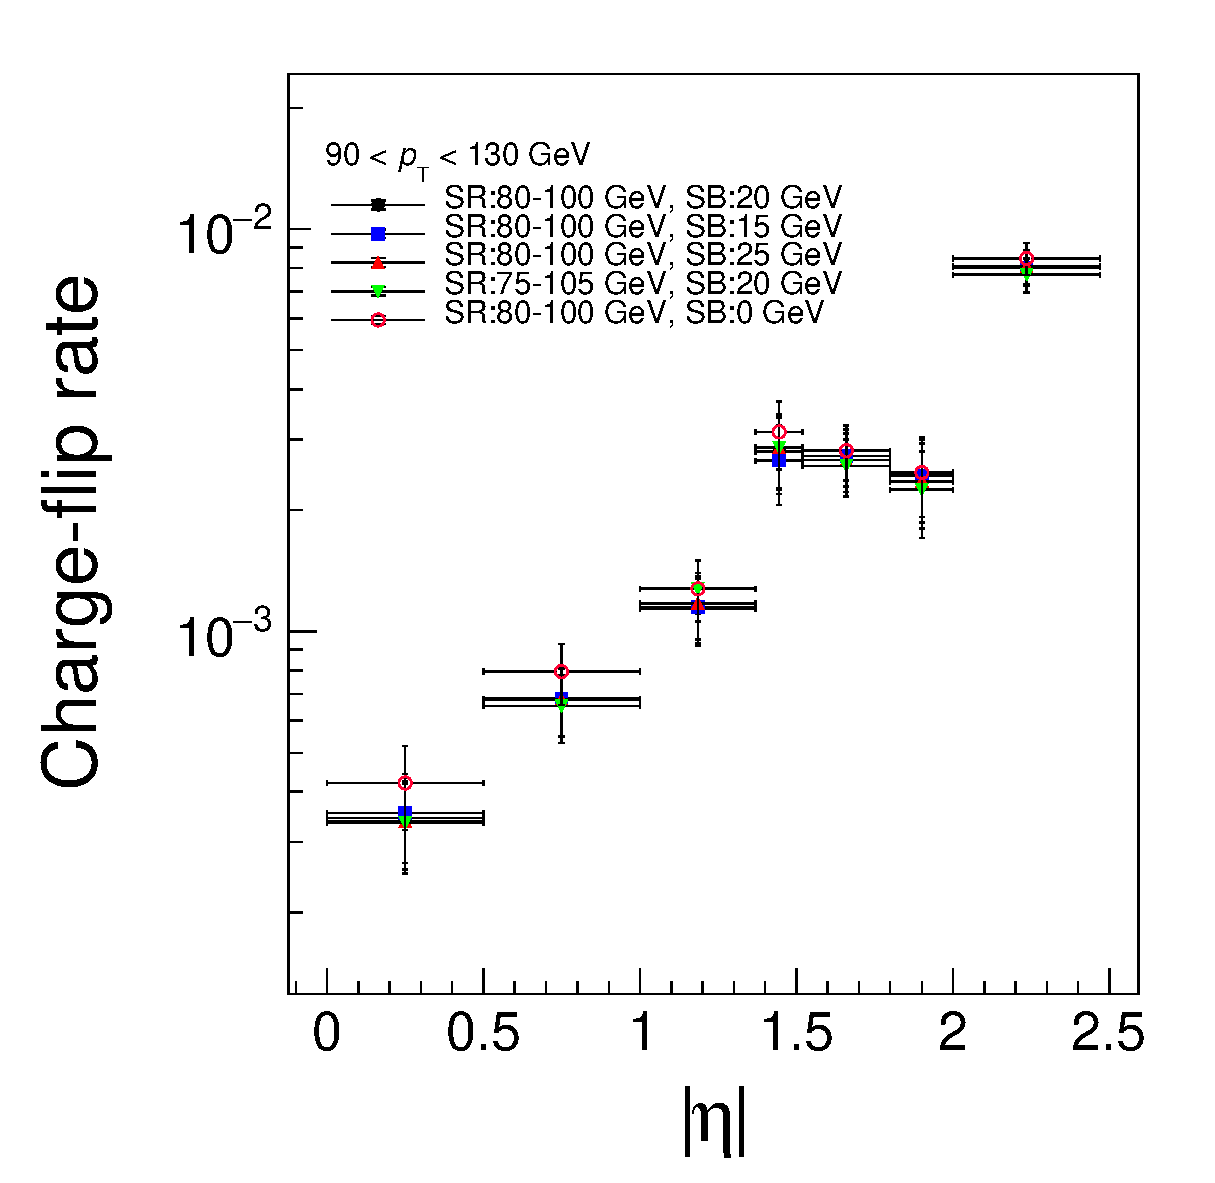
\includegraphics[width=0.3\textwidth]{data/plot/charge_flip/FitPlots/data_cf_comparison_2.eps} \\
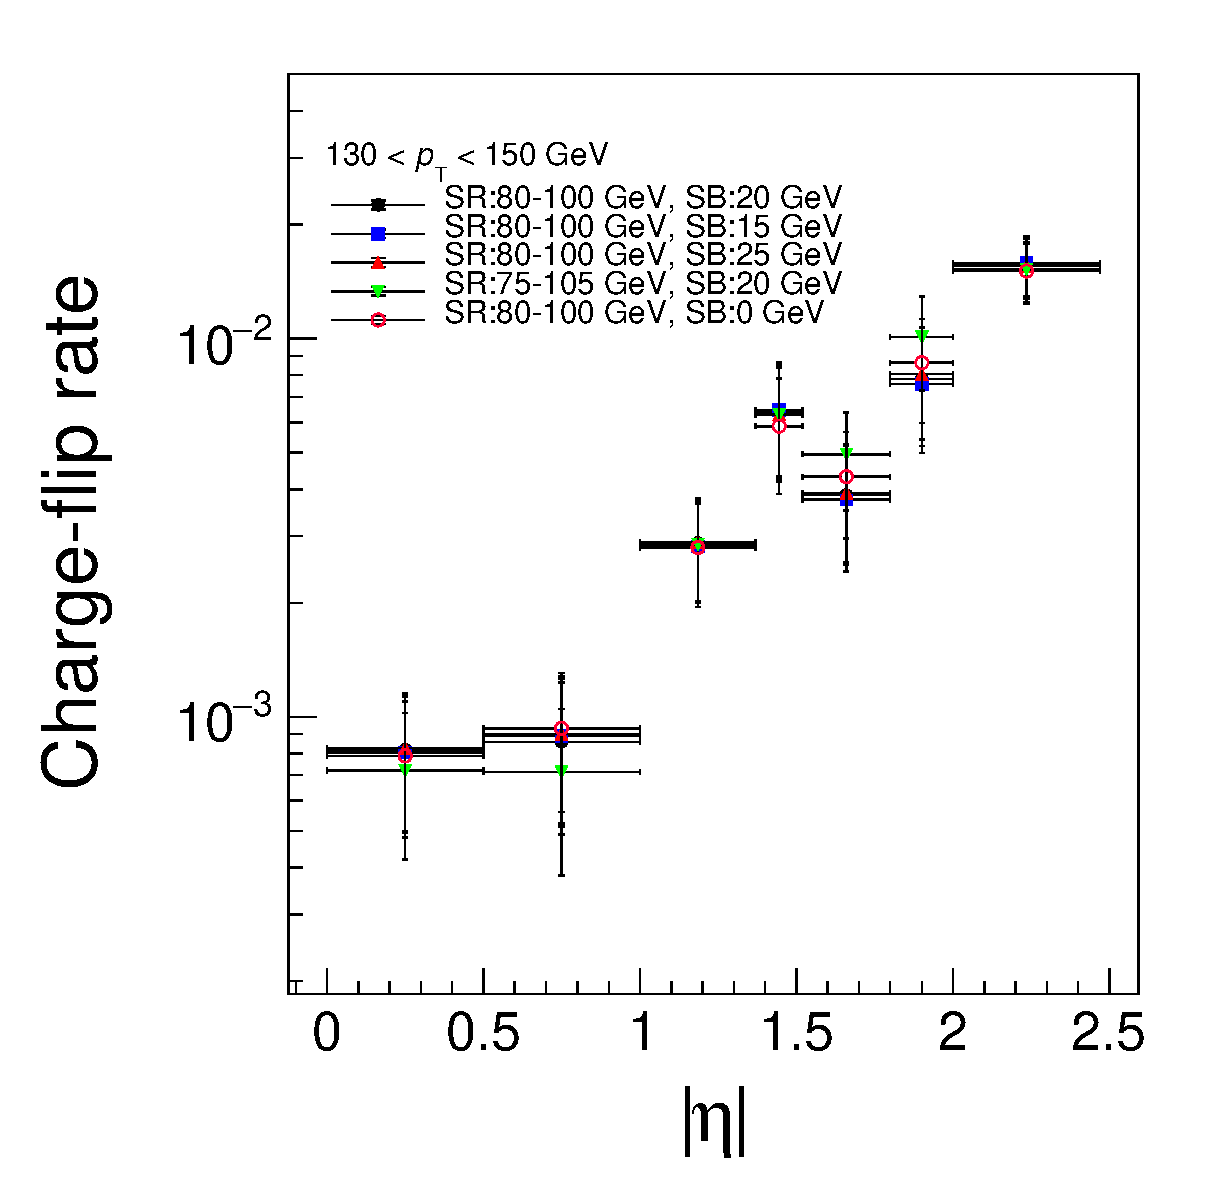
\includegraphics[width=0.3\textwidth]{data/plot/charge_flip/FitPlots/data_cf_comparison_3.eps}
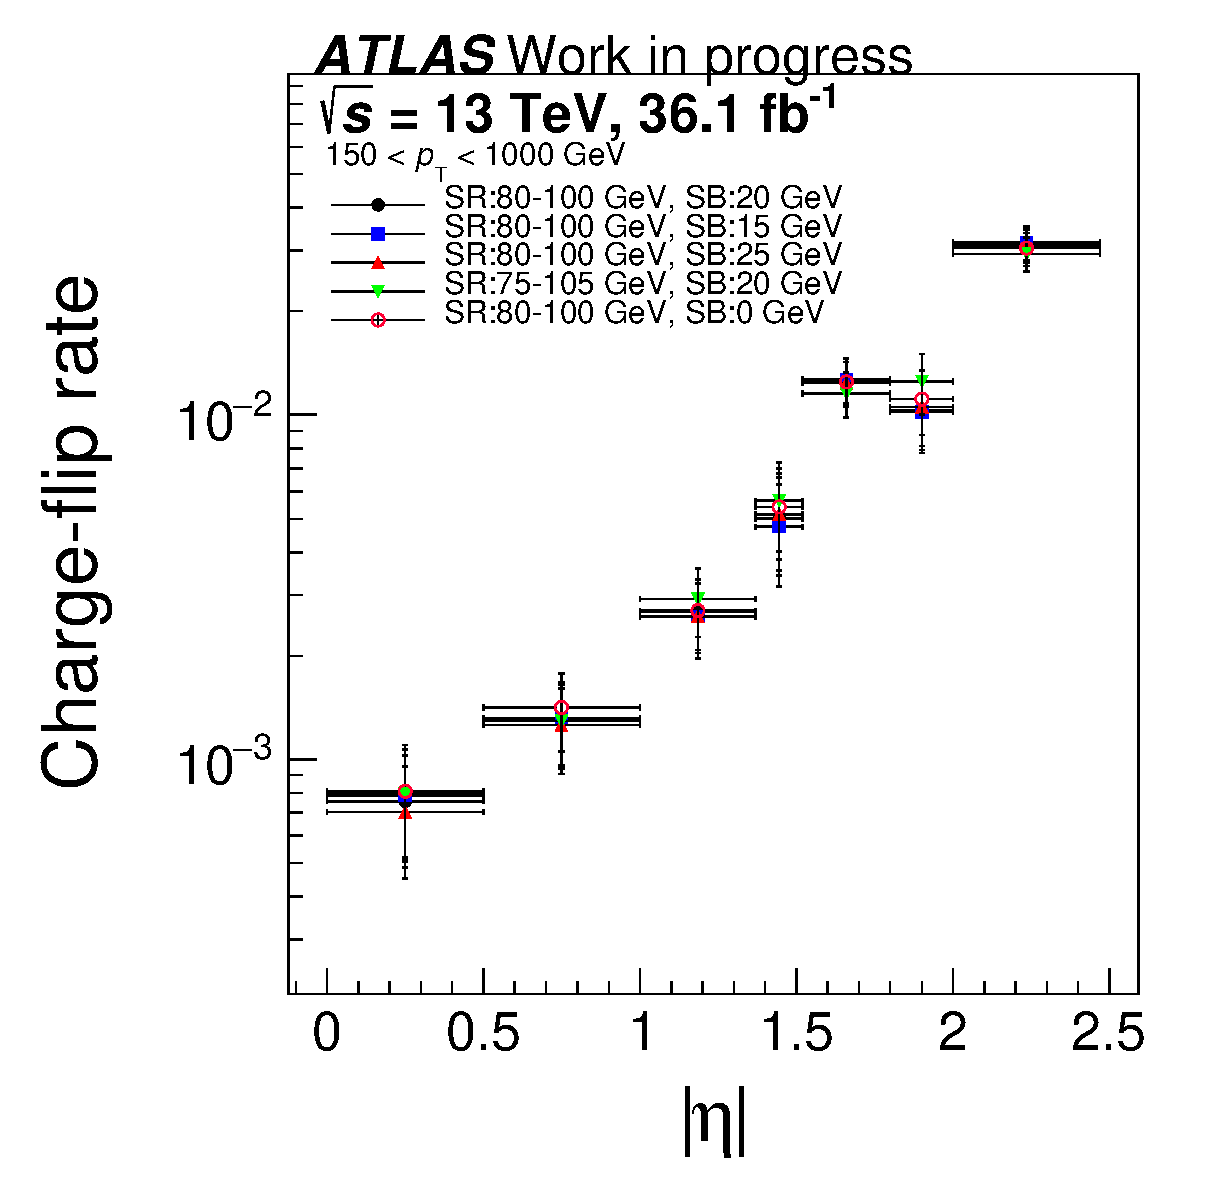
\includegraphics[width=0.3\textwidth]{data/plot/charge_flip/FitPlots/data_cf_comparison_4.eps}
\caption{The systematic variations of the charge-flip rate $\epsilon_i$ in data, due to the background substraction.}
\label{fig:charge_flip_sys_background_substraction}
\end{figure}

\subsection{Systematic uncertainties due to likelihood method}
\label{sec:sys_likelihood}
The systematic uncertainties due to likelihood method are estimated by the difference between the likelihood method and the MC truth method.
In the MC truth method, the charge-flip rate is estimated by using the truth information in $Z \rightarrow ee$ MC samples inside the control region.
The control region requires exactly 2 signal electrons.
The following are the procedures to match the reconstructed electron to the original electron, and hence the original electric charge can be found.
Figure \ref{fig:charge_flip_MC_match} shows how the original electron is found in the decay process described in figure \ref{fig:charge_flip_bremsstrahlung}. In this procedure, some reconstructed electrons will be ignored.
\begin{figure}
\centering
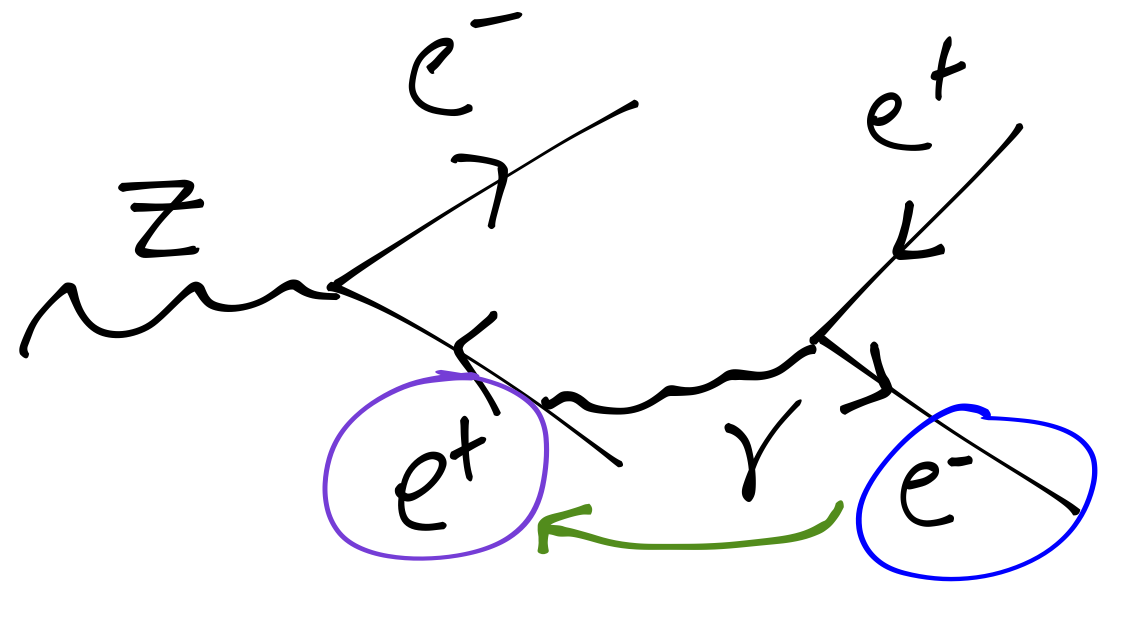
\includegraphics[width=0.5\textwidth]{data/photo/charge_flip/MC-truth.png}
\caption{This diagram shows how the original electron is found through the decay chain.}
\label{fig:charge_flip_MC_match}
\end{figure}
\begin{enumerate}
\item The reconstructed electron will be matched to the truth particle with the smallest $\Delta R$ within the cone $\Delta R < 0.1$. If no any truth particles can be found inside the cone, the reconstructed electron will be ignored.
\item If the truth particle is not an electron, it will be ignored.
\item If the origin of the truth electron is not a Z boson, it will be ignored.
\item If the daughter particle of the Z boson is not an electron, it will be ignored.
\item The charge of the daughter electron from the Z boson is the original charge of the reconstructed electron.
\end{enumerate}

Only the events with two reconstructed electrons that are not ignored in the above procedure are considered.
$N_{\text{total}}$ is the total number of electrons in these events, and $N_{\text{flipped}}$ is the number of electrons that the original charge and the reconstructed charge are different.
By calculating the ratio in each bin, the charge flip rate can be estimated by using the MC truth information.
\begin{equation}
\epsilon_{\text{MC truth}} = \frac{N_{\text{flipped}}}{N_{\text{total}}}
\end{equation}

The systematic uncertainties due to likelihood method $\sigma_{\text{truth}}$ is then given by \\
for MC,
\begin{equation}
\sigma_{\text{truth,MC}} = | \epsilon_{\text{lik,MC}} - \epsilon_{\text{MC truth}} |
\end{equation}
for data,
\begin{equation}
\sigma_{\text{truth,data}} = \epsilon_{\text{lik,data}} \times \frac{\sigma_{\text{truth,MC}}}{\epsilon_{\text{lik,MC}}}
\end{equation}

Figure \ref{fig:charge_flip_sys_truth} shows the comparison of the resulting charge flip rate, between the likelihood method and the MC truth method, by using the $Z \rightarrow ee$ MC samples.
\begin{figure}
\centering
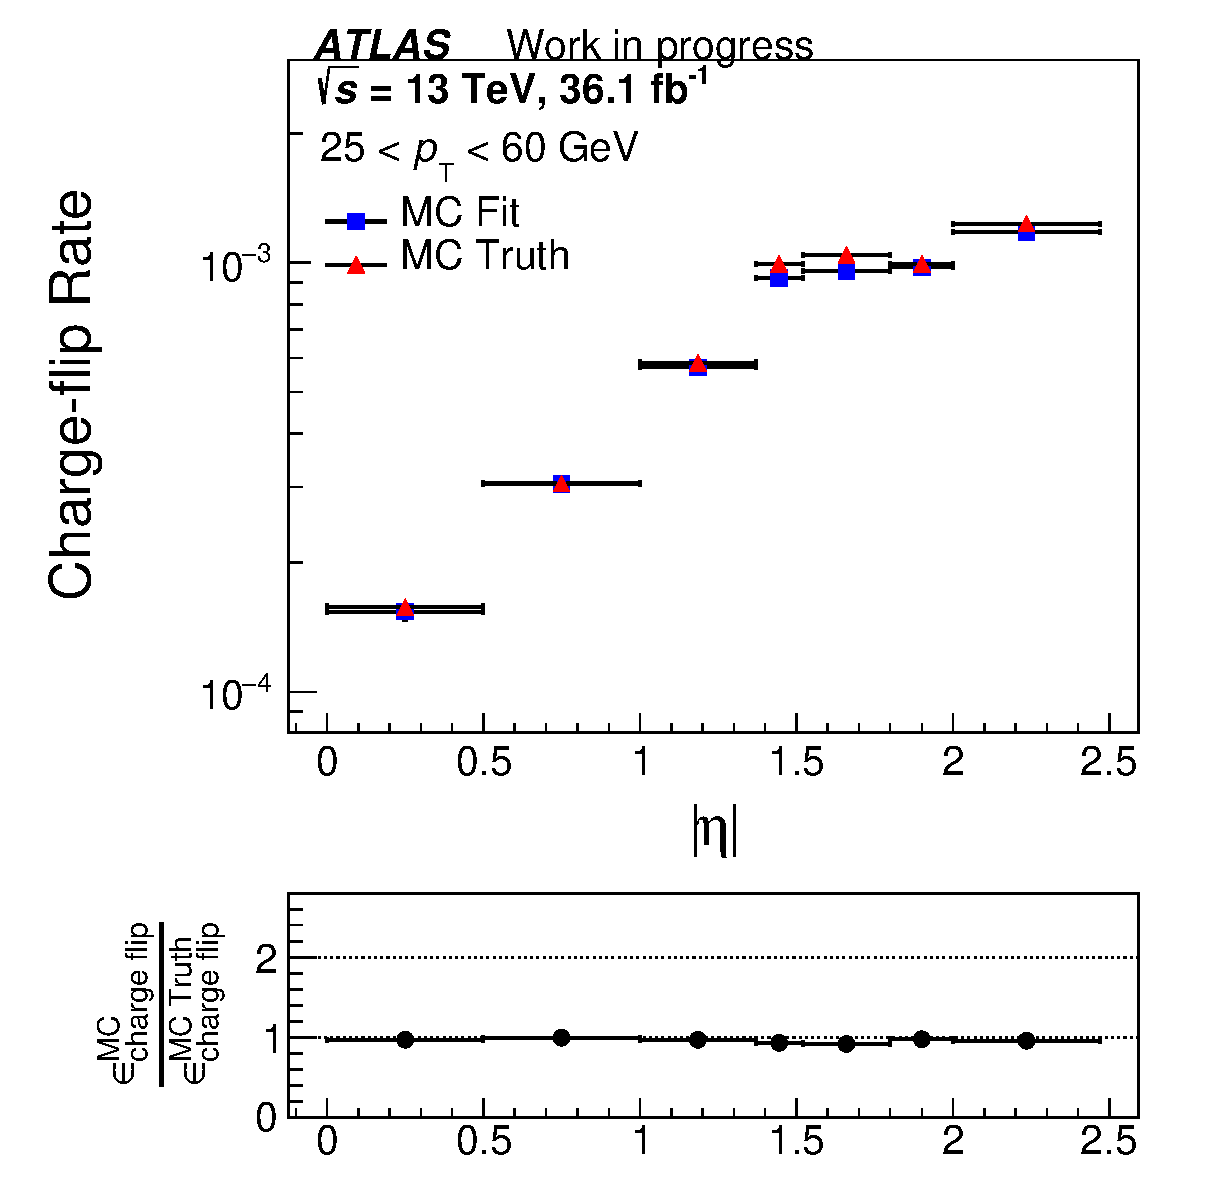
\includegraphics[width=0.3\textwidth]{data/plot/charge_flip/FitPlots/mc_cf_rate_0.eps}
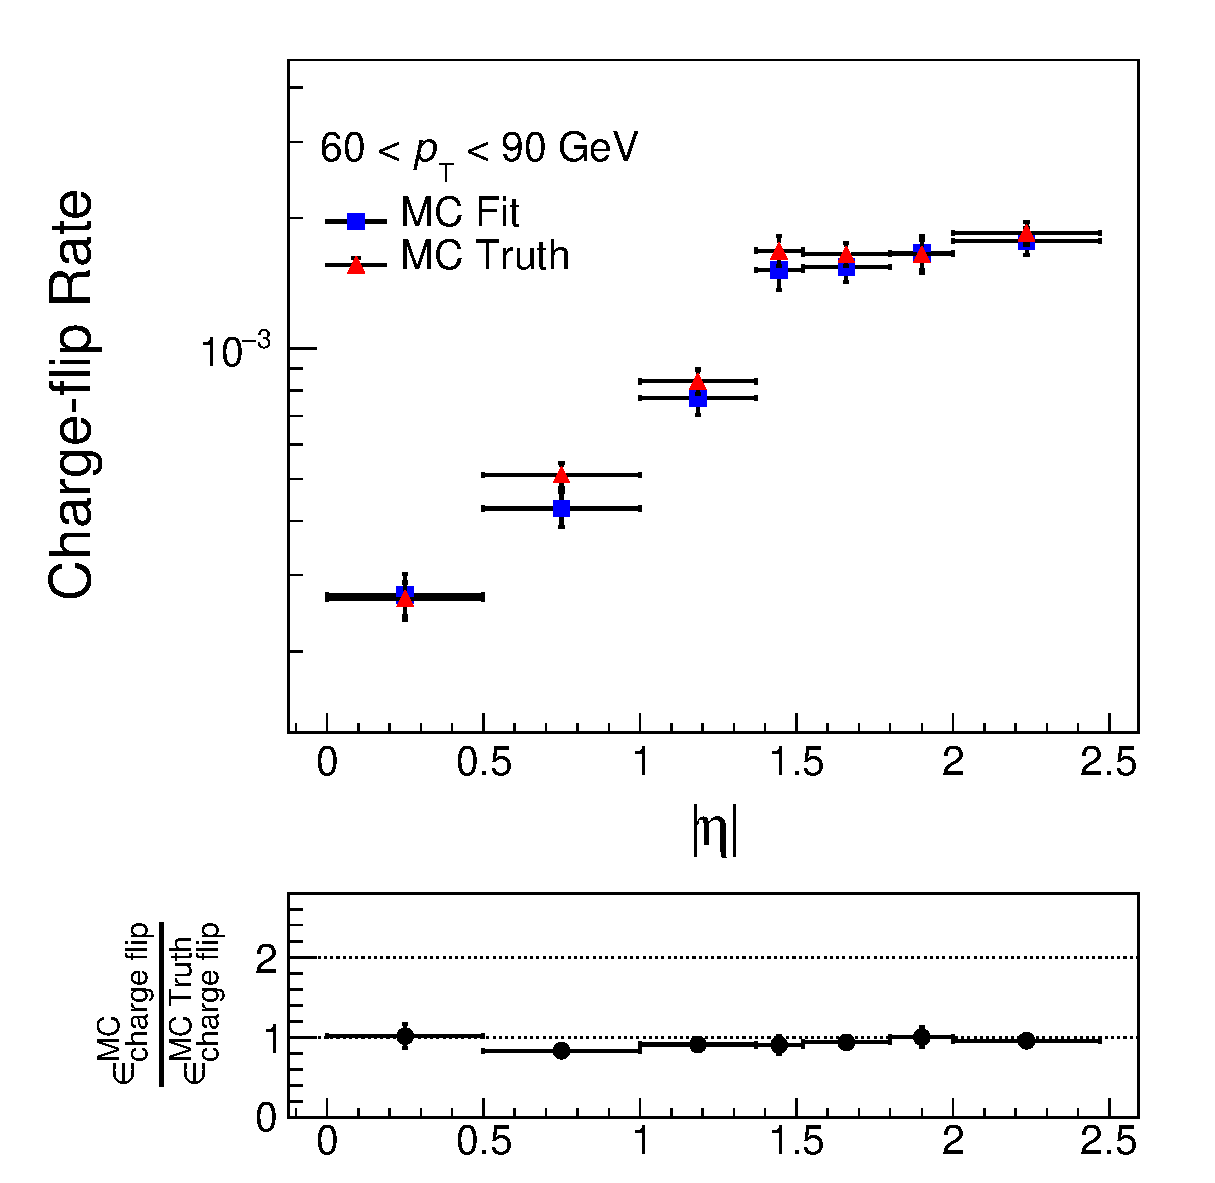
\includegraphics[width=0.3\textwidth]{data/plot/charge_flip/FitPlots/mc_cf_rate_1.eps}
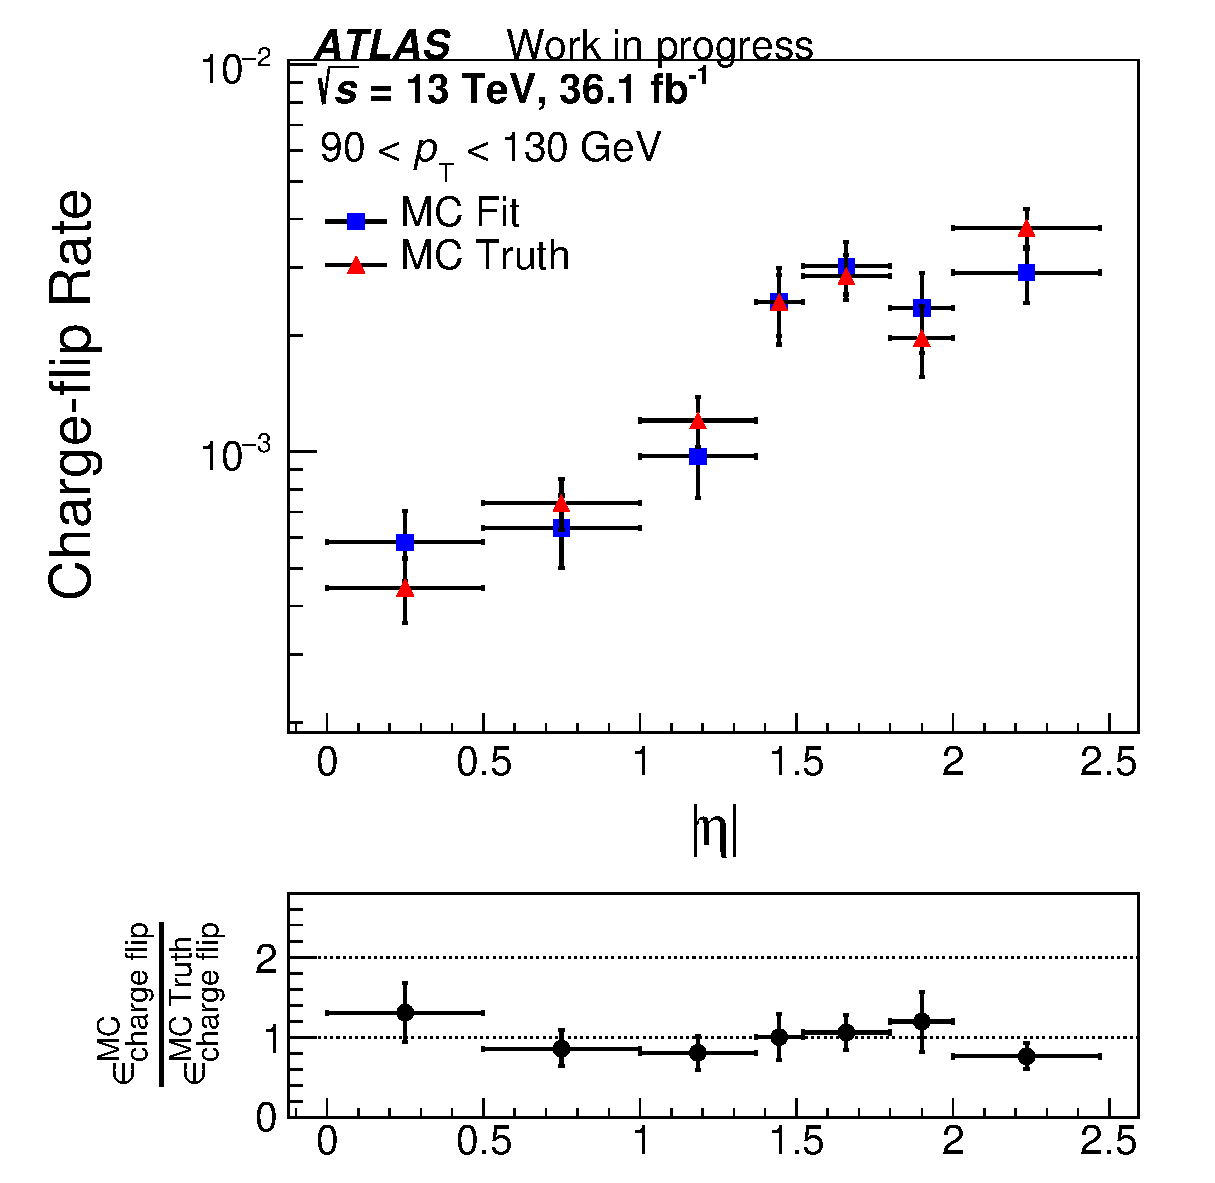
\includegraphics[width=0.3\textwidth]{data/plot/charge_flip/FitPlots/mc_cf_rate_2.eps} \\
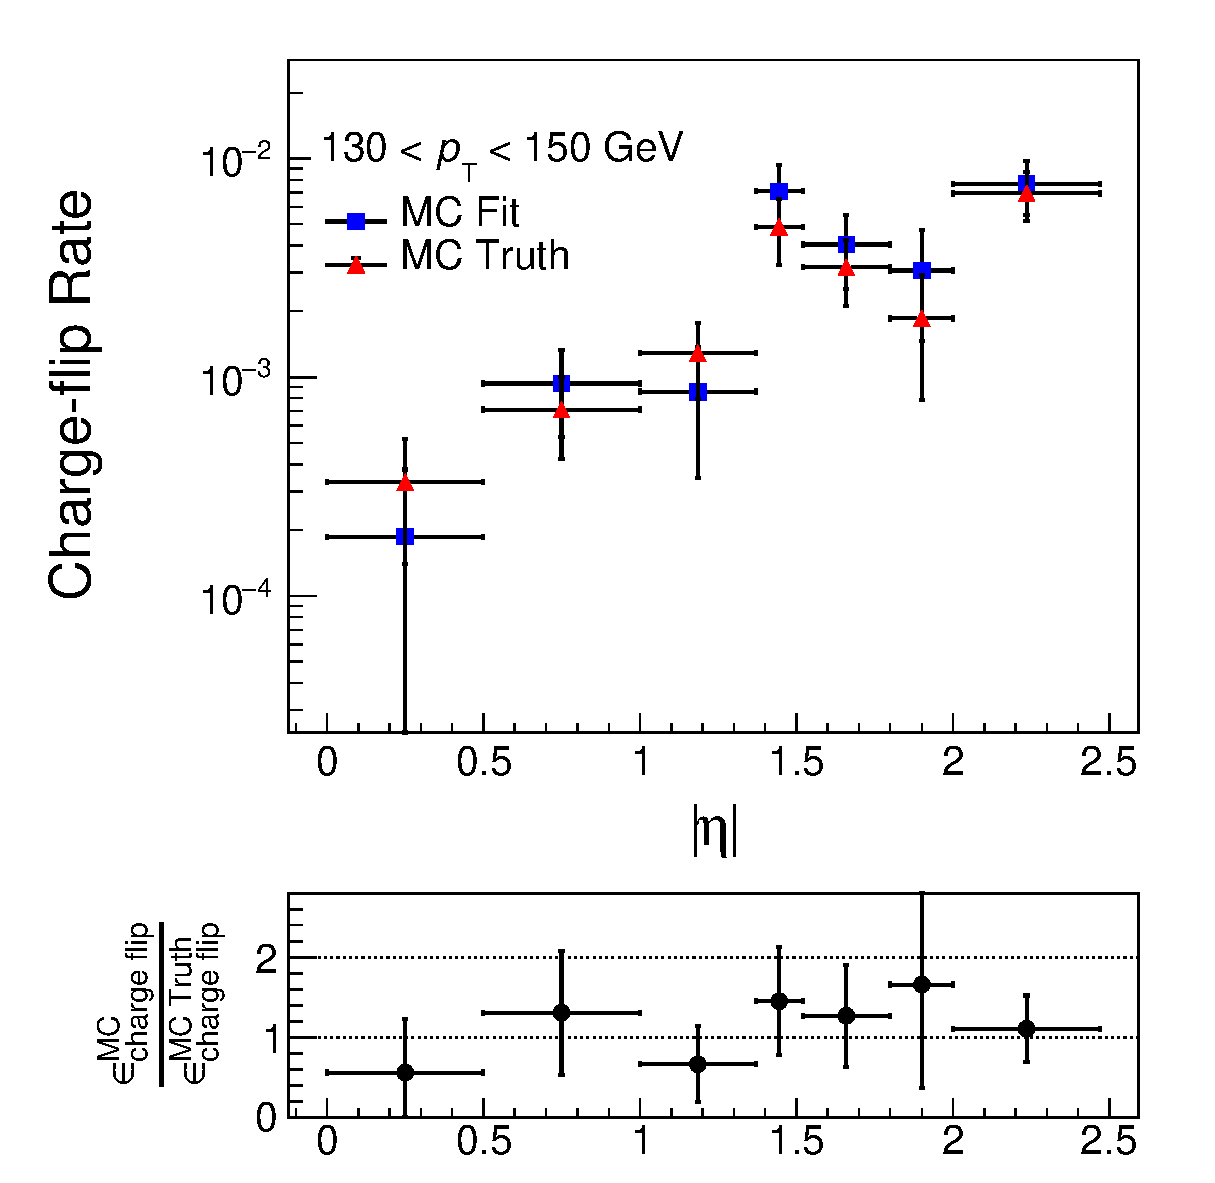
\includegraphics[width=0.3\textwidth]{data/plot/charge_flip/FitPlots/mc_cf_rate_3.eps}
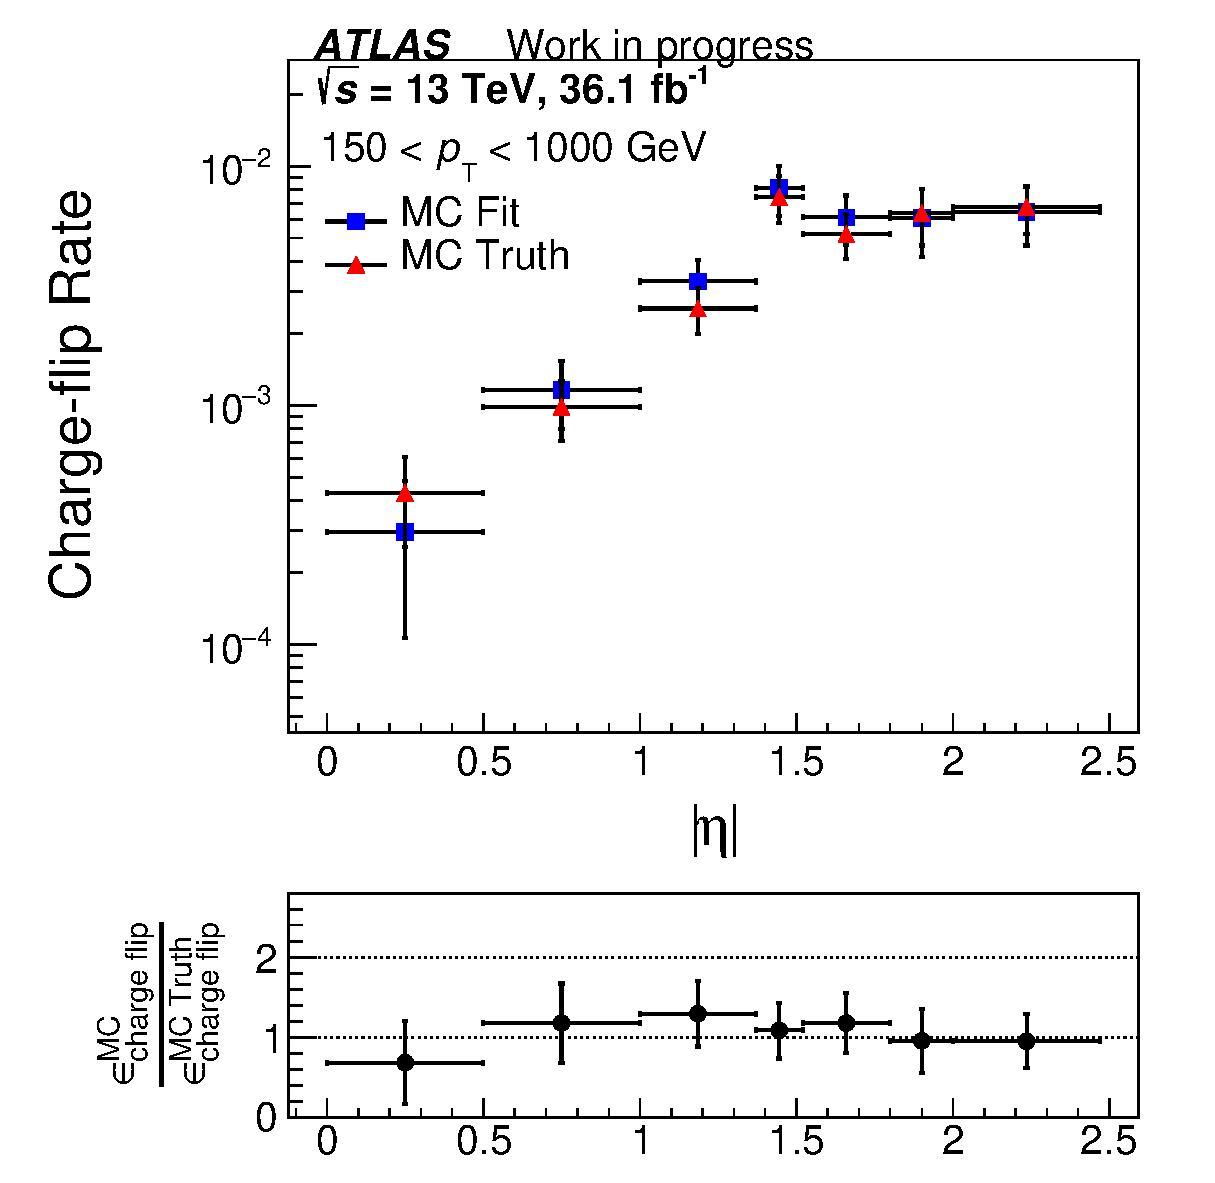
\includegraphics[width=0.3\textwidth]{data/plot/charge_flip/FitPlots/mc_cf_rate_4.eps}
\caption{The comparison between the likelihood method and the MC truth method, by using the $Z \rightarrow ee$ MC samples. Hence, the systematic uncertainties due to likelihood method can be estimated.}
\label{fig:charge_flip_sys_truth}
\end{figure}

\subsection{Results with total uncertainties}
\label{sec:charge_flip_results_stat}
The total systematic uncertainties is the quadratic sum of systematic uncertainties due to the background substraction and the likelihood method, described in section \ref{sec:sys_background_substraction} and \ref{sec:sys_likelihood} respectively.
\begin{equation}
\sigma_{\text{sys}} = \sqrt{\sigma_{\text{bgk}} ^2+ \sigma_{\text{truth}} ^2}
\end{equation}
The total uncertainties is the quadratic sum of the total systematic uncertainties and the statistical uncertainties in the likelihood method.
\begin{equation}
\sigma_{\text{tot}} = \sqrt{\sigma_{\text{sys}} ^2 + \sigma_{\text{lik}} ^2}
\label{equ:tot_error}
\end{equation}

Figure \ref{fig:charge_flip_data_tot} shows the measured values of the charge-flip rate $\epsilon_i$ by using the data, with total uncertainties described in equation \ref{equ:tot_error}.

\begin{figure}
\centering
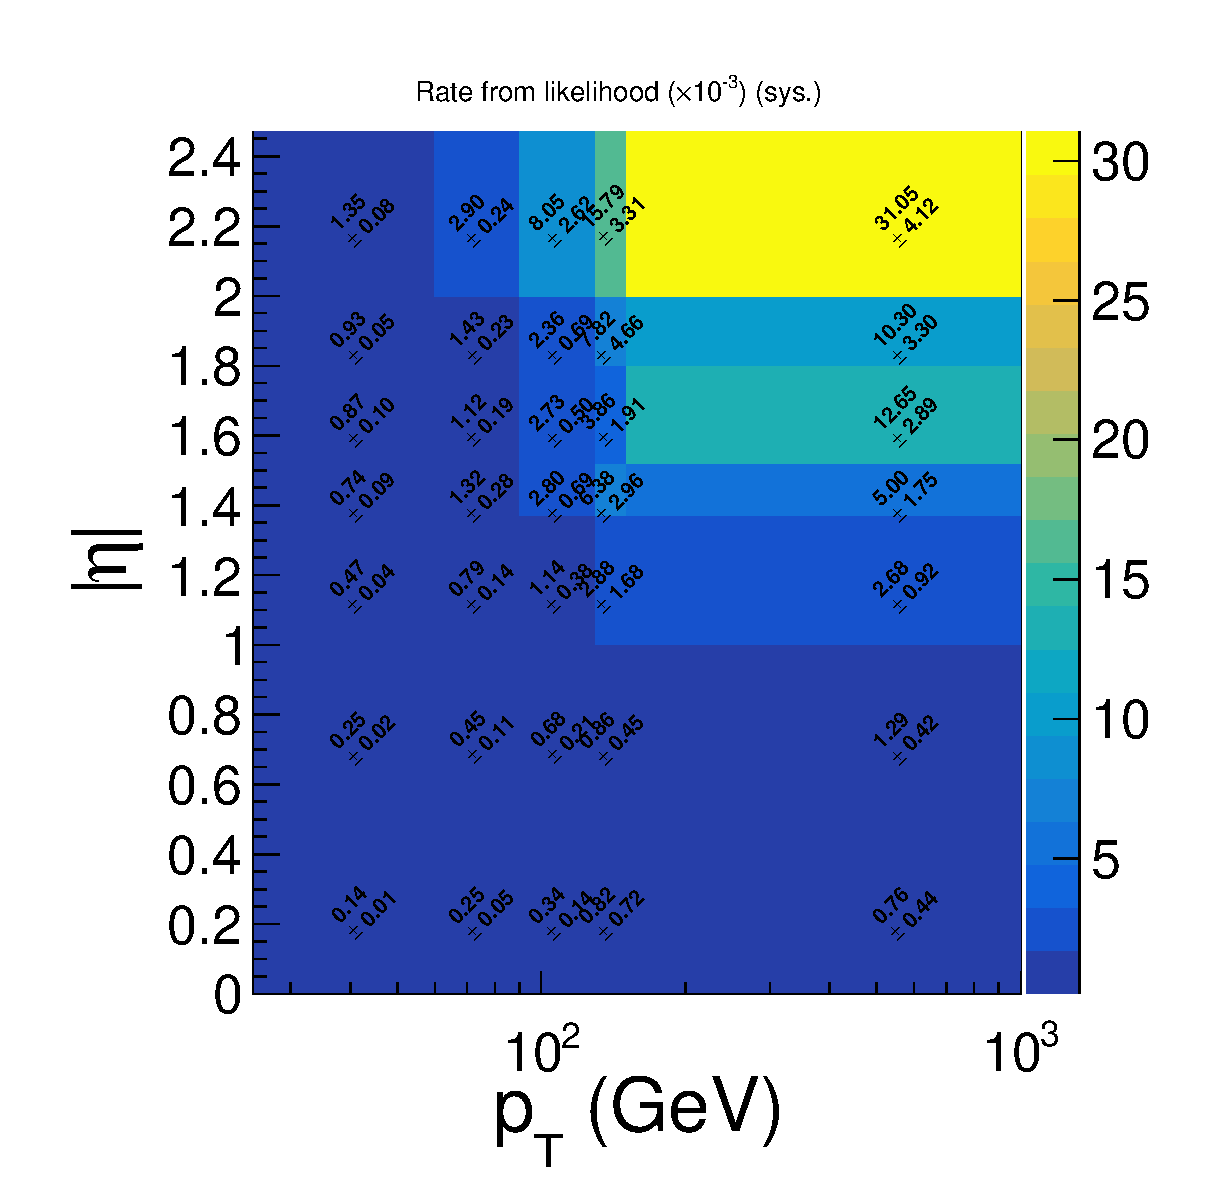
\includegraphics[width=\textwidth]{data/plot/charge_flip/FitPlots/data_cf_rate_tot.eps}
\caption{The measured values of the charge-flip rate $\epsilon_i$ in data, with total uncertainties.}
\label{fig:charge_flip_data_tot}
\end{figure}

\subsection{MC validation}
\label{sec:charge_flip_MC_validation}
The charge flip rate can be validated by using the $Z \rightarrow ee$ MC samples.
By using the equation \ref{equ:mapp1} and \ref{equ:NSS3}, $N^{ij}_{SS}$ can be approximated by
\begin{align}
N^{ij}_{SS} &= [ \epsilon_i (1-\epsilon_j) + (1-\epsilon_i) \epsilon_j ] m^{ij}_{OS} \\
&\approx [ \epsilon_i (1-\epsilon_j) + (1-\epsilon_i) \epsilon_j ] \frac{ M^{ij}_{OS} }{ (1-\epsilon_i) (1-\epsilon_j) } \\
&= \frac{\epsilon_i (1-\epsilon_j) + (1-\epsilon_i) \epsilon_j}{(1-\epsilon_i) (1-\epsilon_j)} M^{ij}_{OS}
\end{align}
Also, in the equation \ref{equ:MSS}, $m^{ij}_{SS}$ is zero for the $Z \rightarrow ee$ MC samples, we have
\begin{align}
M^{ij}_{SS} &= \epsilon_i (1-\epsilon_j) m^{ij}_{OS} + (1-\epsilon_i) \epsilon_j m^{ij}_{OS} \\
&= N^{ij}_{SS}
\end{align}
Hence, it is expected that
\begin{align}
M^{ij}_{SS} \approx \frac{\epsilon_i (1-\epsilon_j) + (1-\epsilon_i) \epsilon_j}{(1-\epsilon_i) (1-\epsilon_j)} M^{ij}_{OS}
\end{align}
By weighting the OS events in MC with the weight,
\begin{align}
\text{weight} = \frac{\epsilon_i (1-\epsilon_j) + (1-\epsilon_i) \epsilon_j}{(1-\epsilon_i) (1-\epsilon_j)}
\end{align}
the weighted OS events and the SS events will be close to each other.
This can be used to validate the charge flip rate.
Figure shows the comparison between the weighted OS events and the SS events, with different variables.
All event weights are applied, except the charge flip scale factor.
The weighted OS events and the SS events agree within the uncertainties.
\begin{figure}
\centering
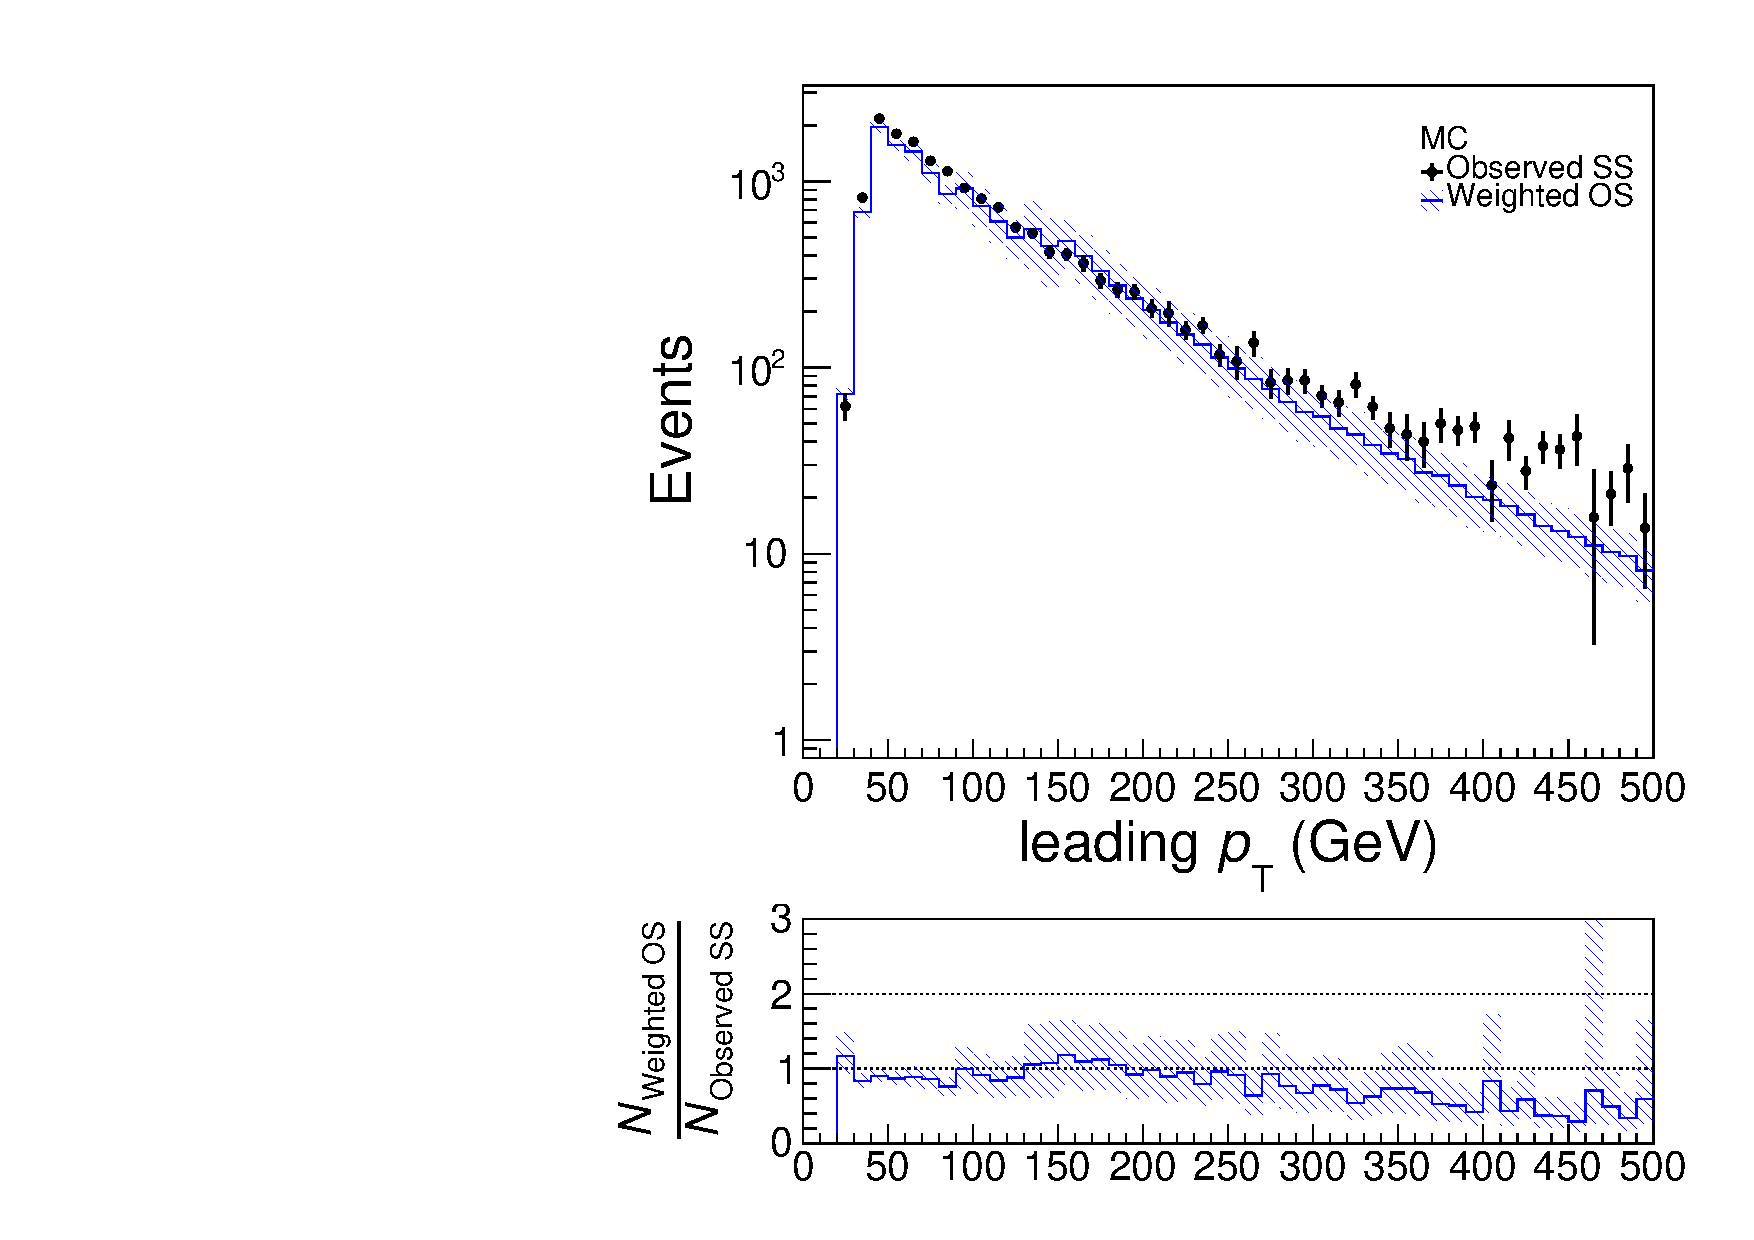
\includegraphics[width=0.3\textwidth]{data/plot/charge_flip/ReweightPlots/plots_NOchfSF/mc_pt_1.pdf}
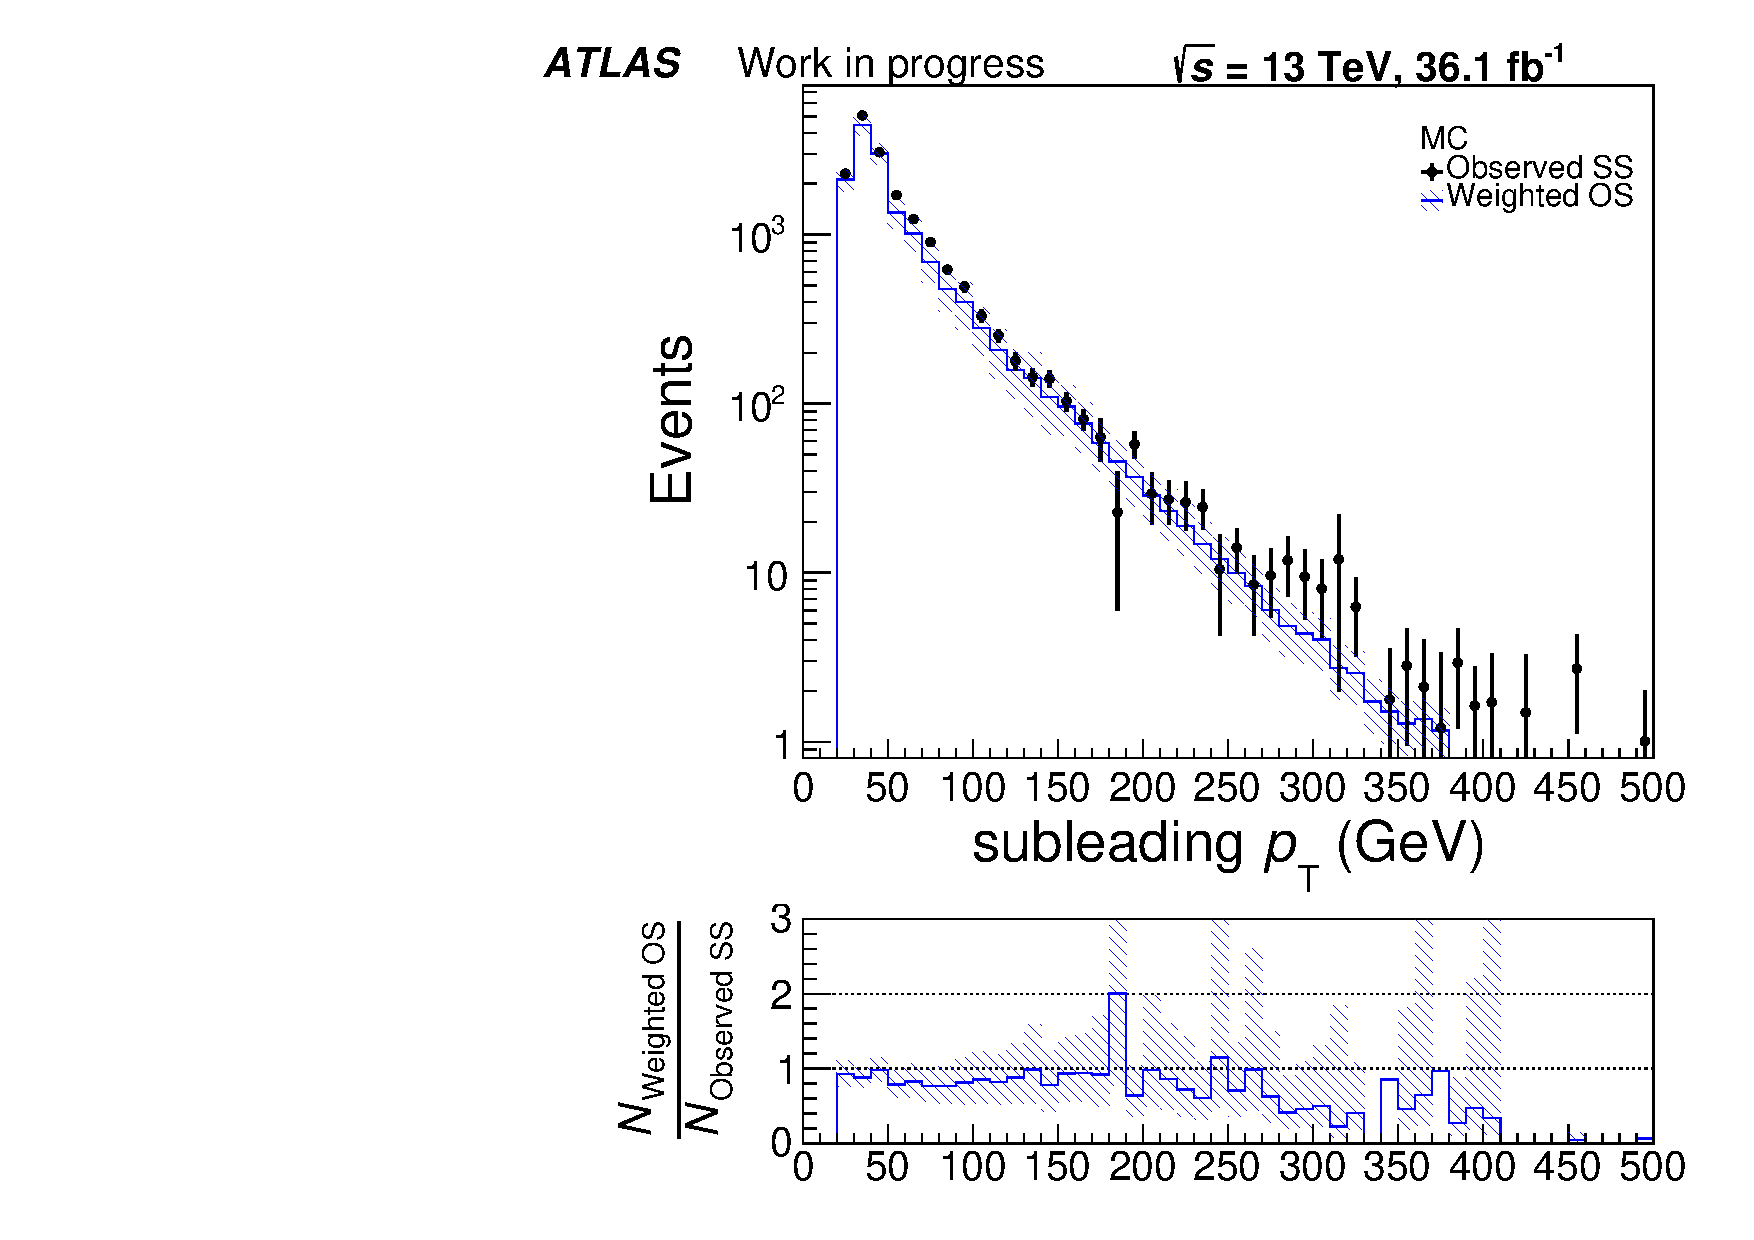
\includegraphics[width=0.3\textwidth]{data/plot/charge_flip/ReweightPlots/plots_NOchfSF/mc_pt_2.pdf} \\
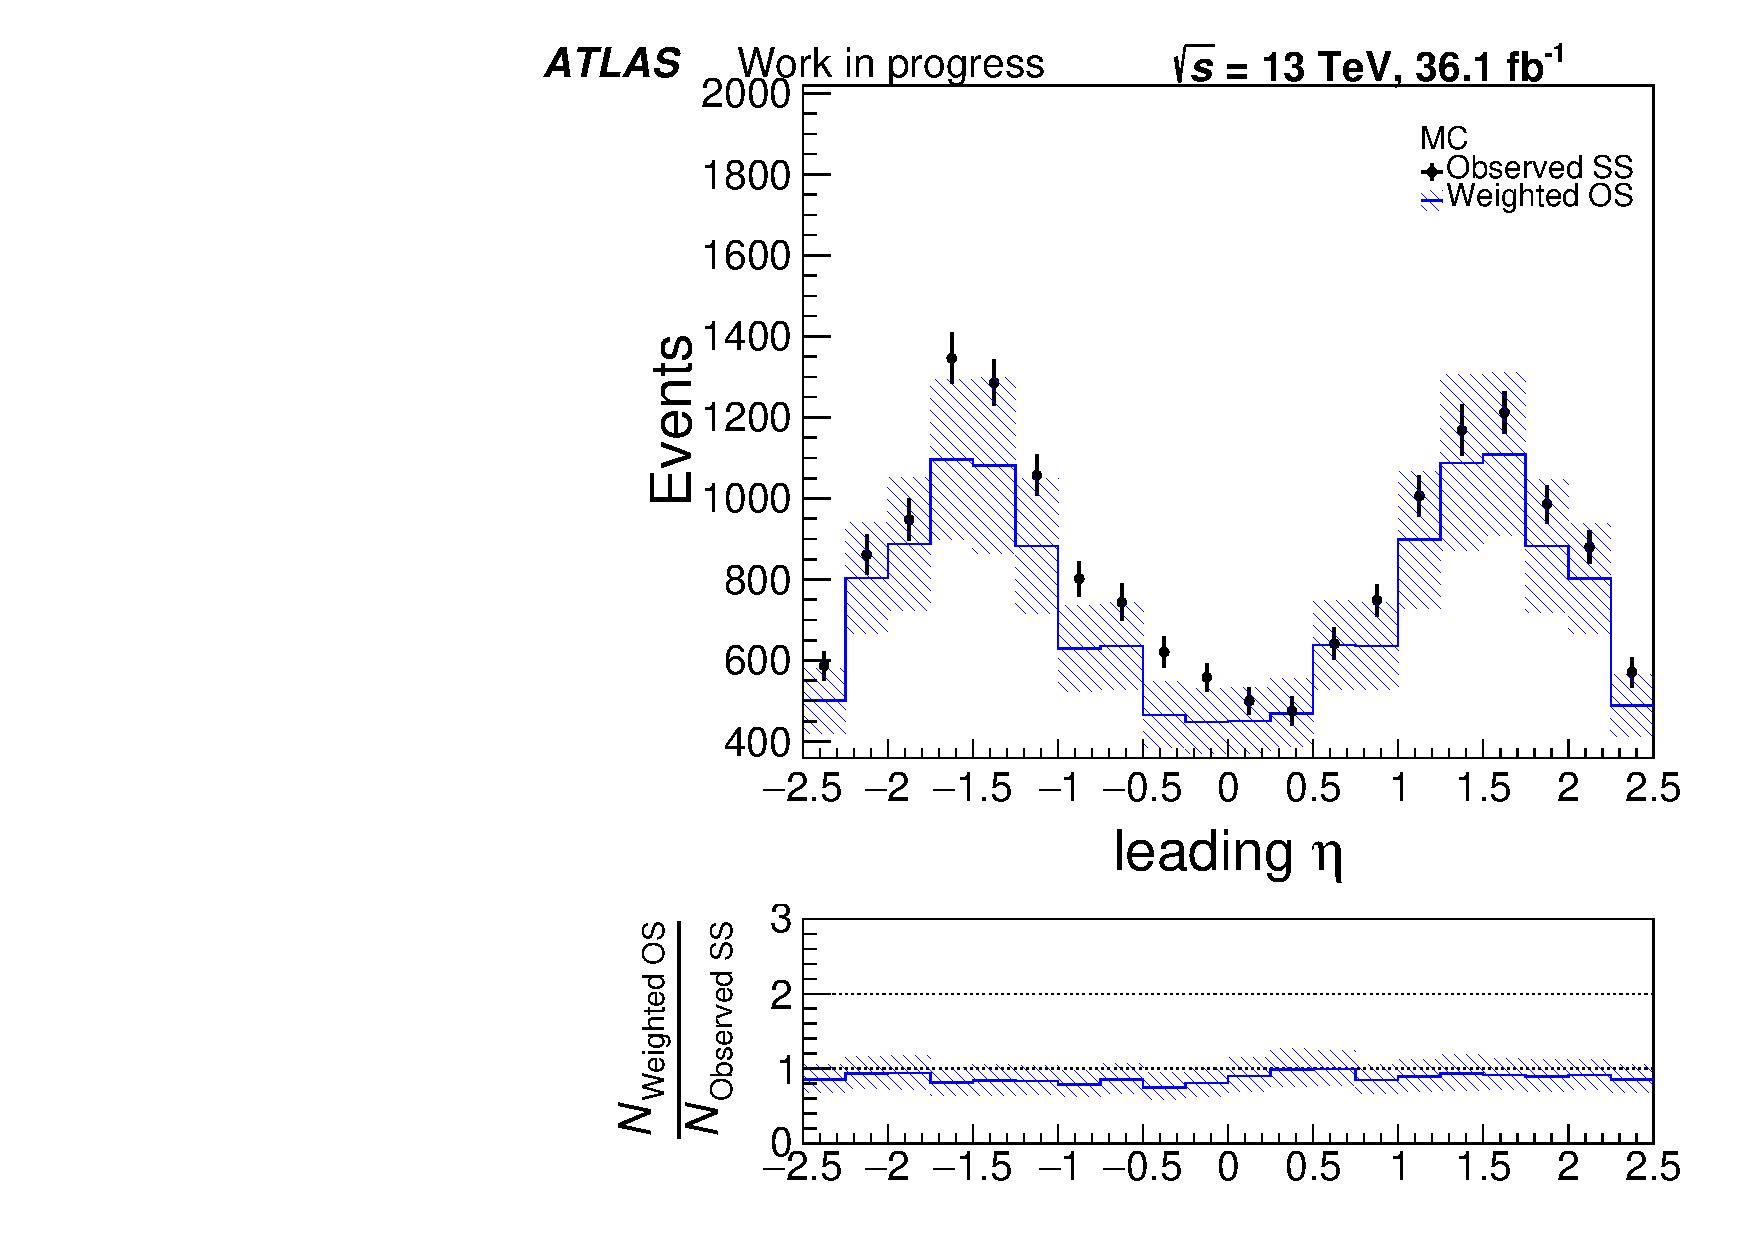
\includegraphics[width=0.3\textwidth]{data/plot/charge_flip/ReweightPlots/plots_NOchfSF/mc_eta_1.pdf}
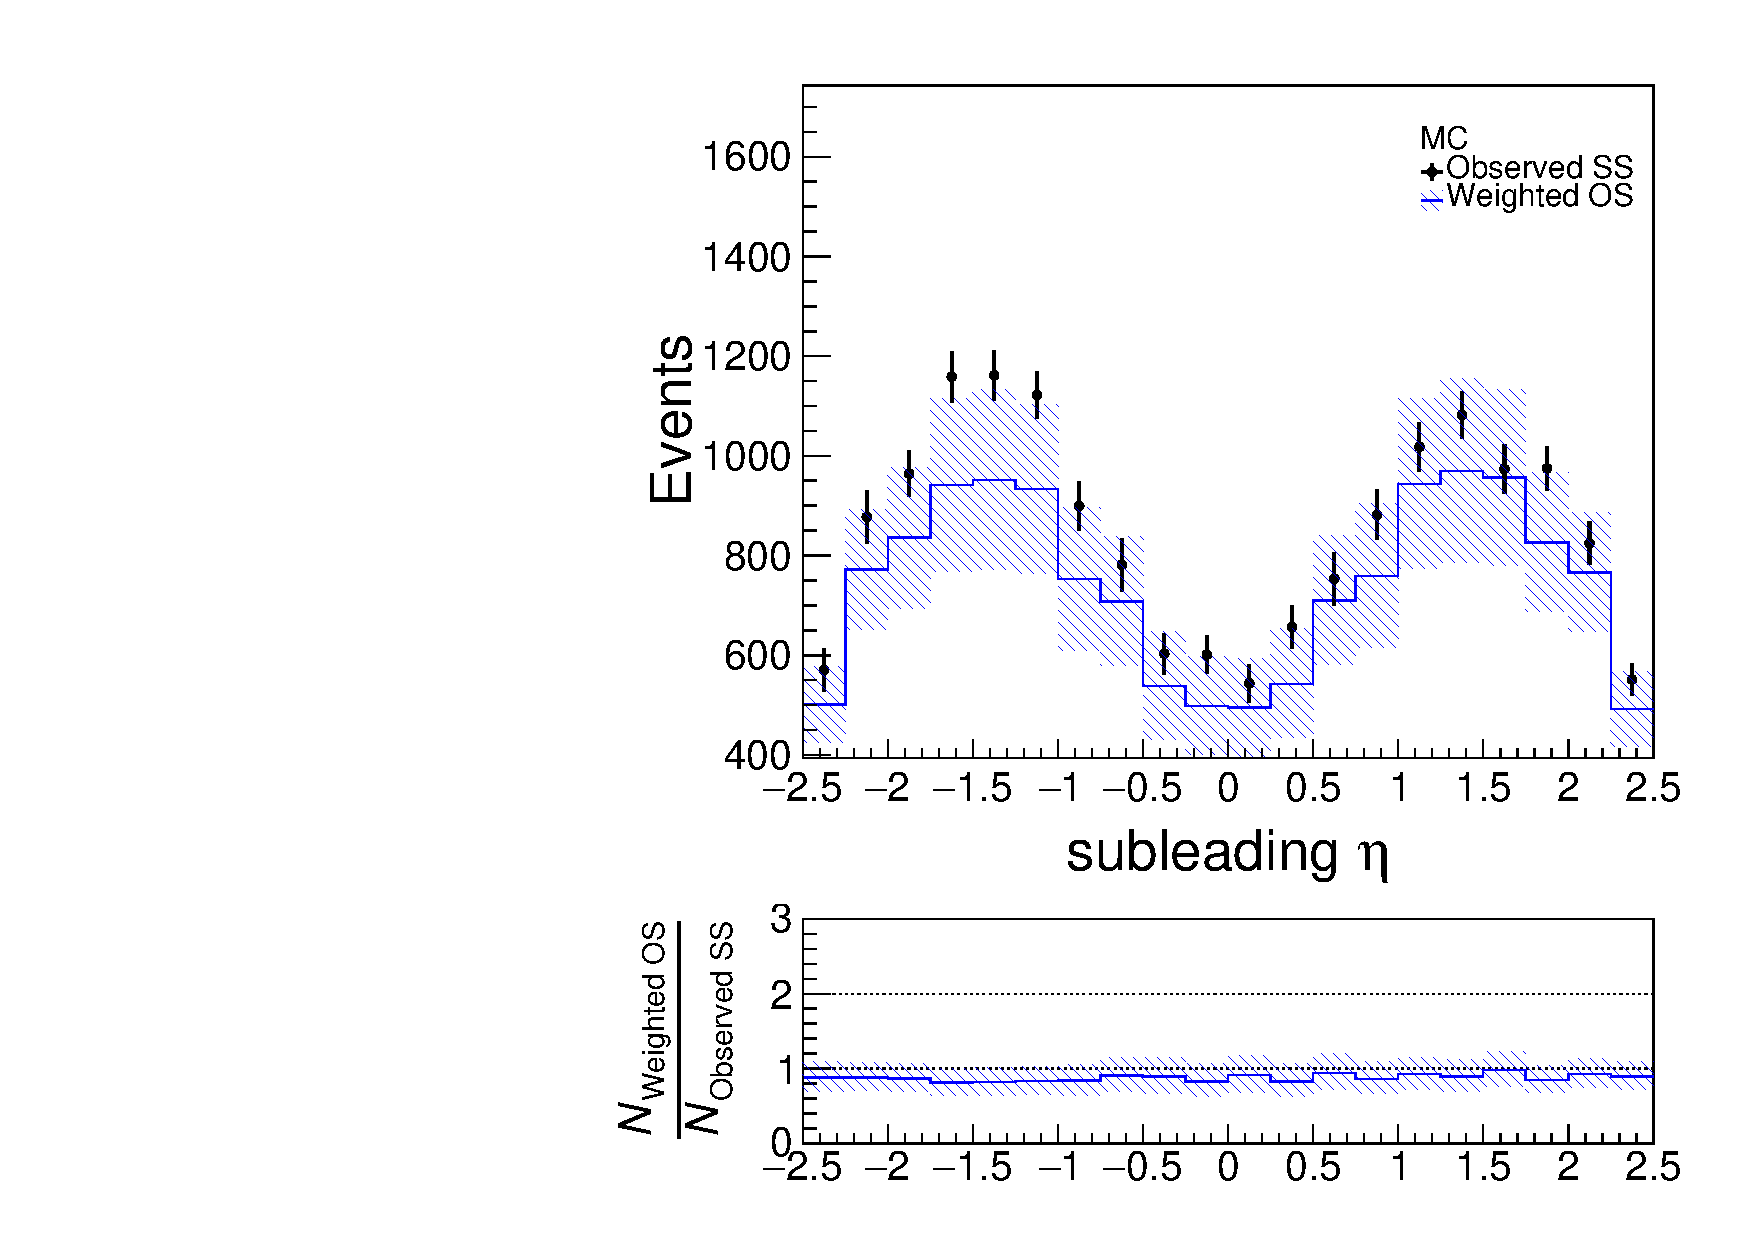
\includegraphics[width=0.3\textwidth]{data/plot/charge_flip/ReweightPlots/plots_NOchfSF/mc_eta_2.pdf} \\
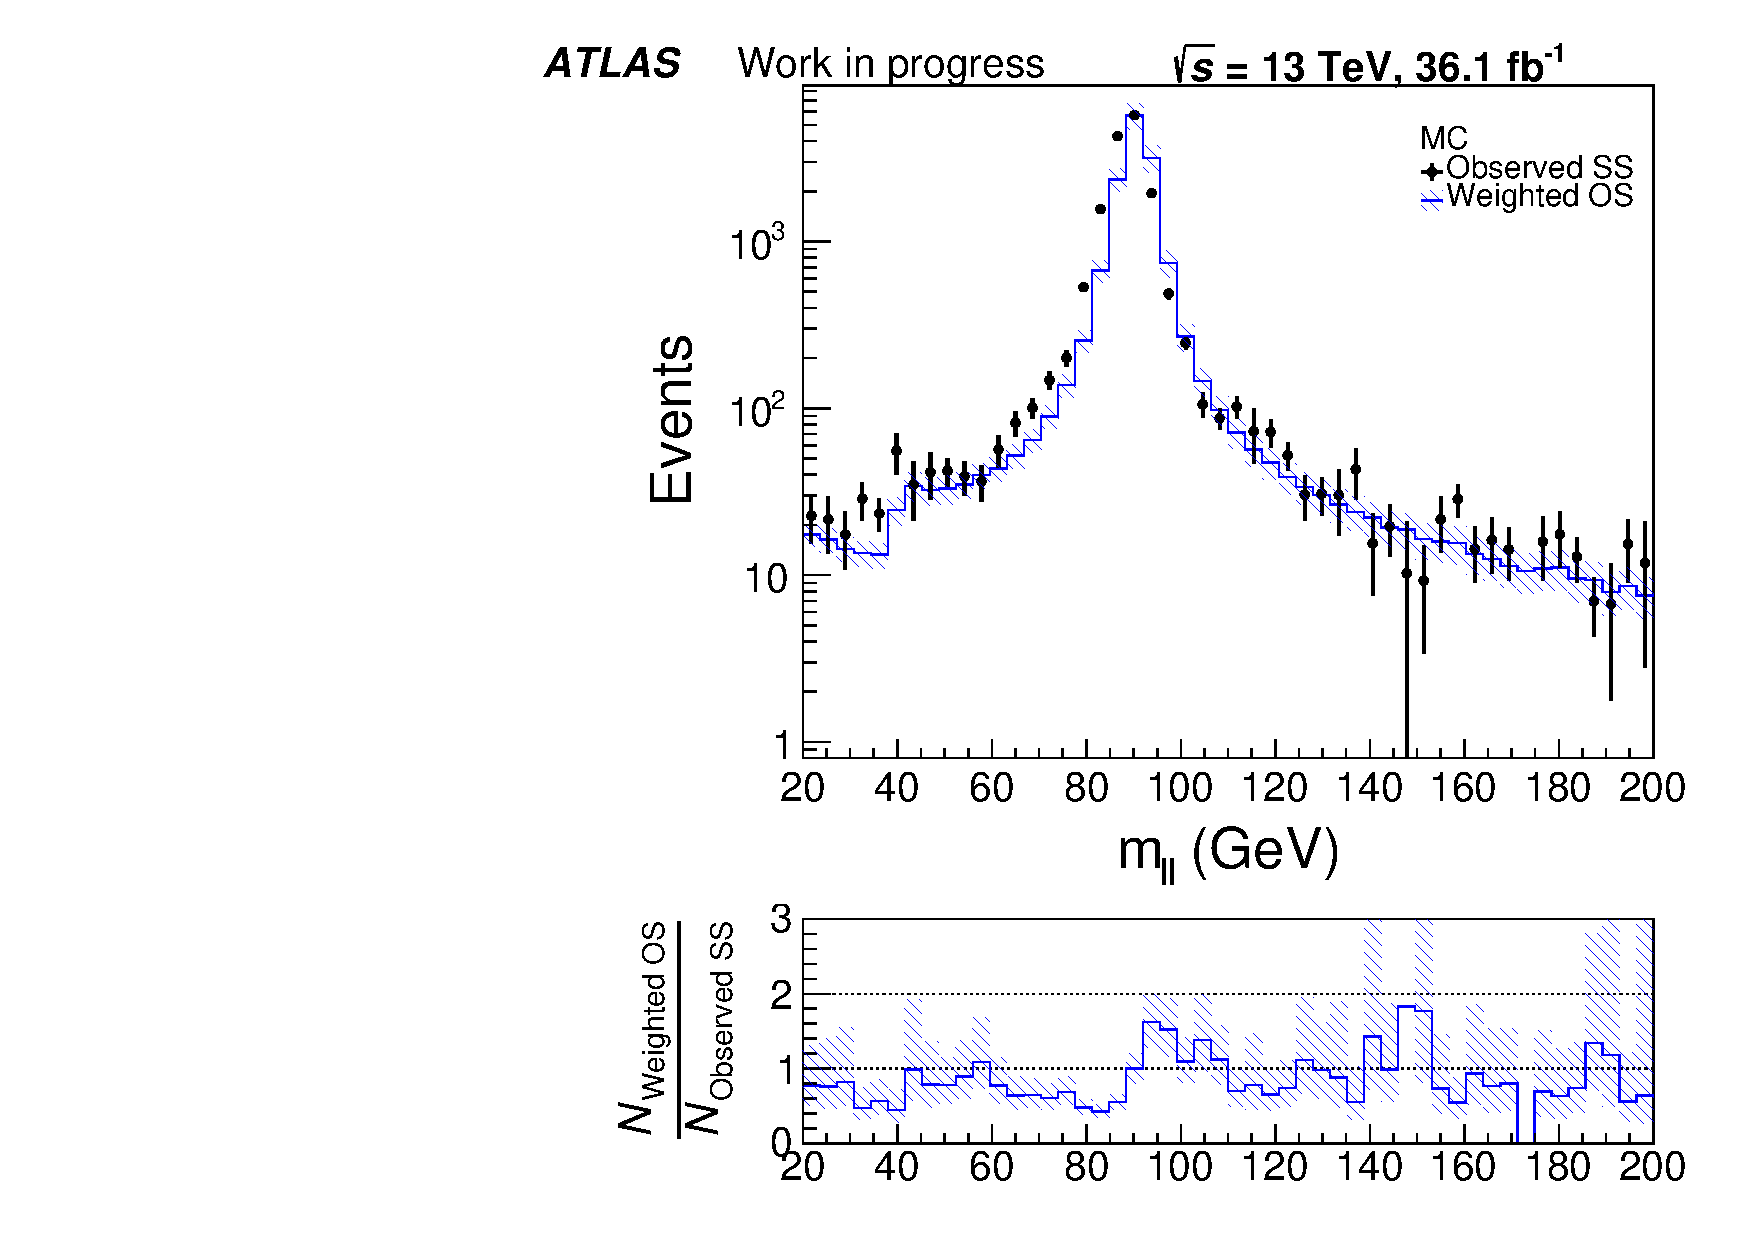
\includegraphics[width=0.3\textwidth]{data/plot/charge_flip/ReweightPlots/plots_NOchfSF/mc_mll.pdf}
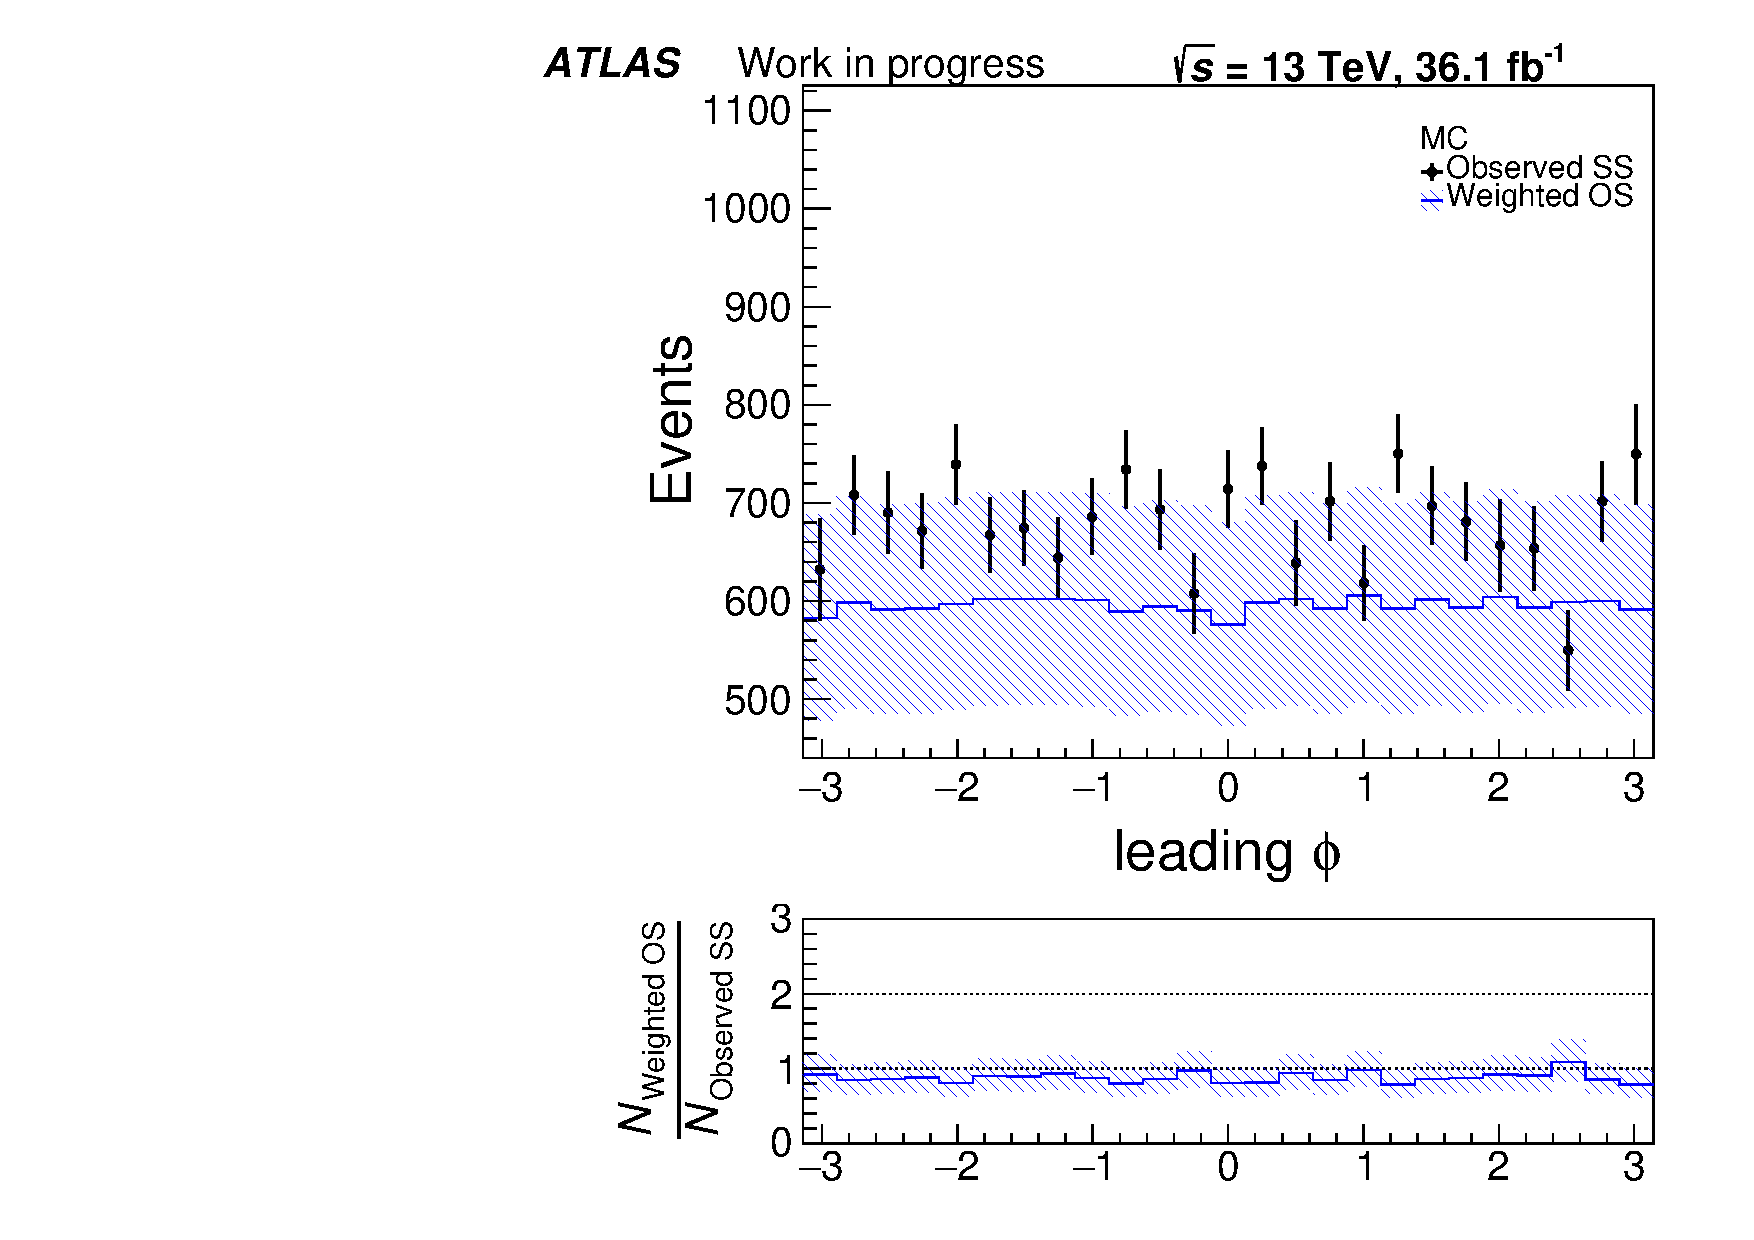
\includegraphics[width=0.3\textwidth]{data/plot/charge_flip/ReweightPlots/plots_NOchfSF/mc_phi_1.pdf}
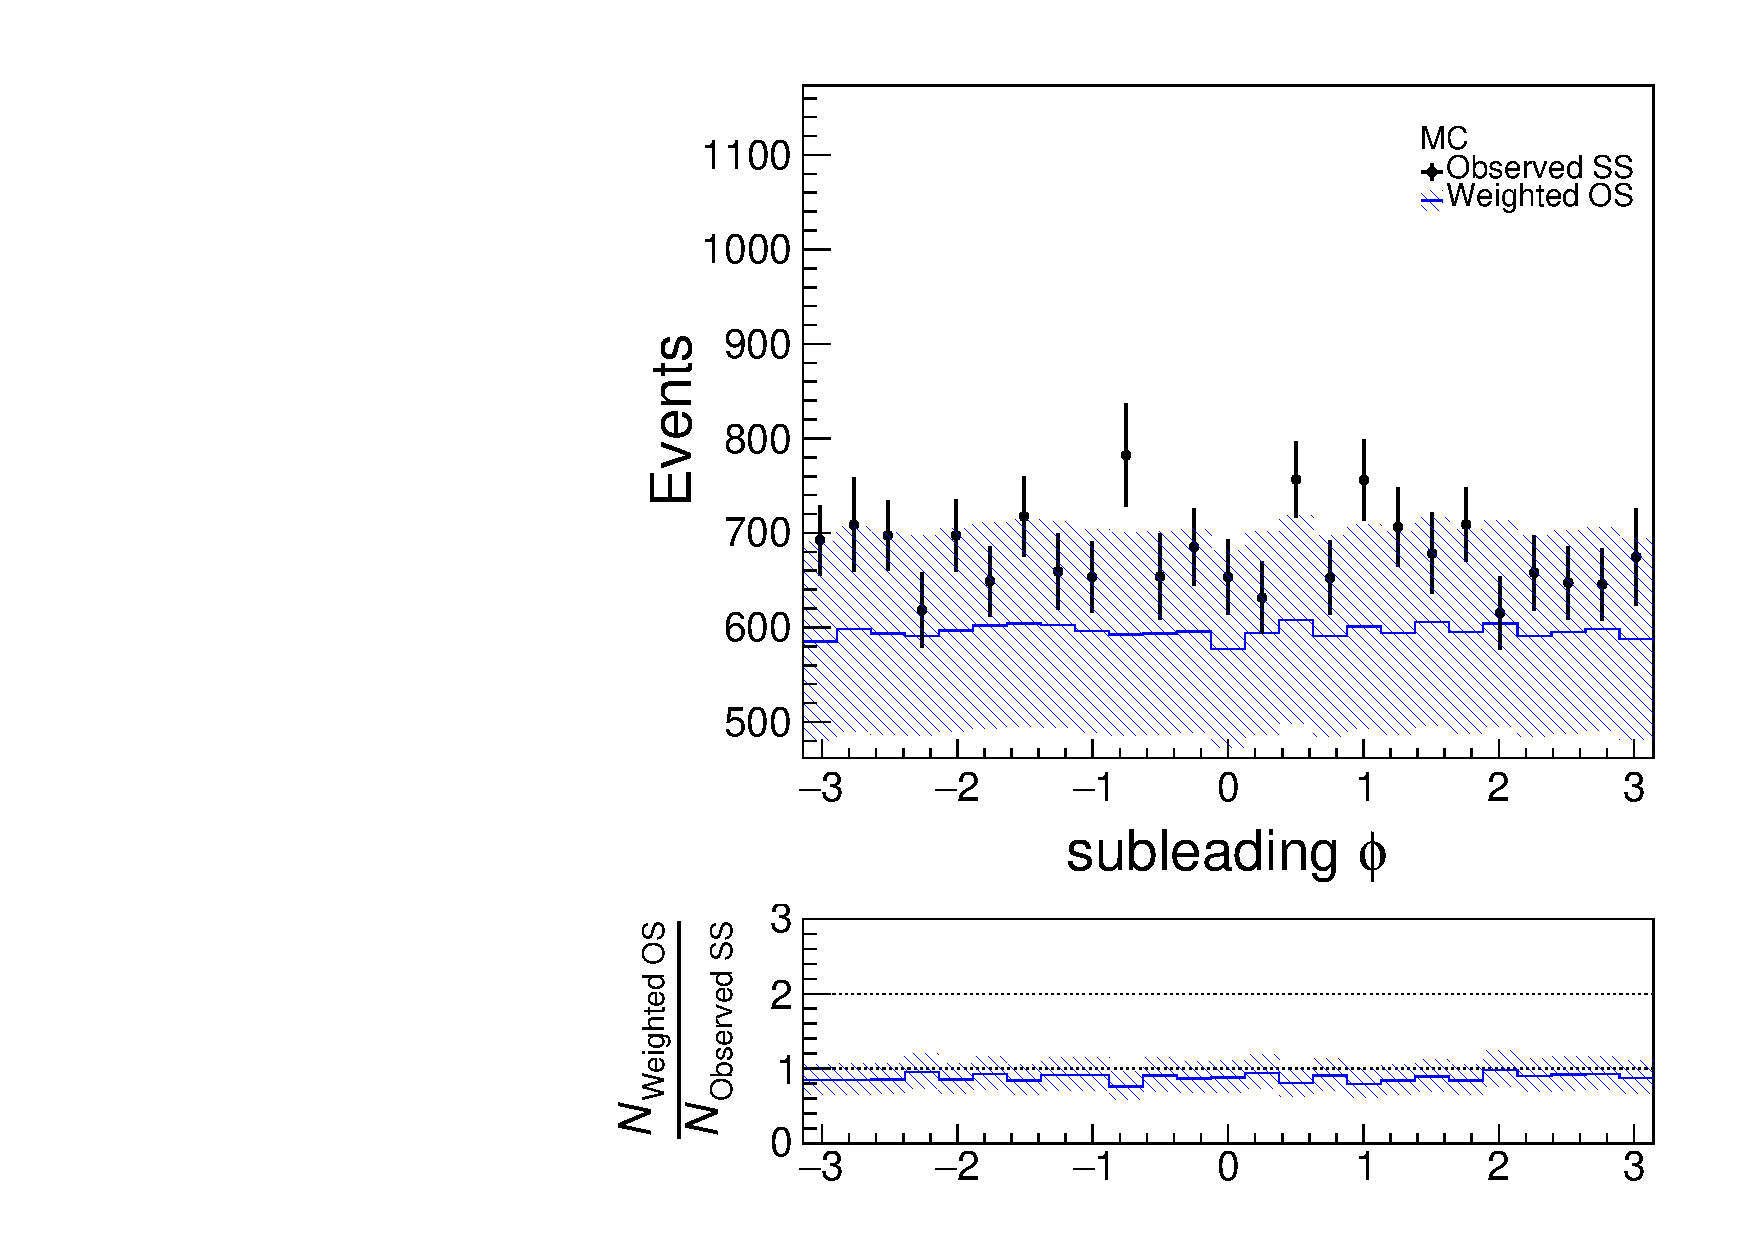
\includegraphics[width=0.3\textwidth]{data/plot/charge_flip/ReweightPlots/plots_NOchfSF/mc_phi_2.pdf}
\caption{The comparison between the weighted OS events and the SS events, with different variables.}
\end{figure}

\section{fake lepton background}
